\documentclass[a4paper]{book}
\usepackage{a4wide}
\usepackage{makeidx}
\usepackage{graphicx}
\usepackage{multicol}
\usepackage{float}
\usepackage{listings}
\usepackage{color}
\usepackage{textcomp}
\usepackage{alltt}
\usepackage{times}
\usepackage{ifpdf}
\ifpdf
\usepackage[pdftex,
            pagebackref=true,
            colorlinks=true,
            linkcolor=blue,
            unicode
           ]{hyperref}
\else
\usepackage[ps2pdf,
            pagebackref=true,
            colorlinks=true,
            linkcolor=blue,
            unicode
           ]{hyperref}
\usepackage{pspicture}
\fi
\usepackage[utf8]{inputenc}
\usepackage{doxygen}
\lstset{language=C++,inputencoding=utf8,basicstyle=\footnotesize,breaklines=true,breakatwhitespace=true,tabsize=8,numbers=left }
\makeindex
\setcounter{tocdepth}{3}
\renewcommand{\footrulewidth}{0.4pt}
\begin{document}
\hypersetup{pageanchor=false}
\begin{titlepage}
\vspace*{7cm}
\begin{center}
{\Large opendaq \\[1ex]\large basic }\\
\vspace*{1cm}
{\large Generated by Doxygen 1.7.1}\\
\vspace*{0.5cm}
{\small Thu Oct 28 2010 21:58:52}\\
\end{center}
\end{titlepage}
\clearemptydoublepage
\pagenumbering{roman}
\tableofcontents
\clearemptydoublepage
\pagenumbering{arabic}
\hypersetup{pageanchor=true}
\chapter{Class Index}
\section{Class Hierarchy}
This inheritance list is sorted roughly, but not completely, alphabetically:\begin{DoxyCompactList}
\item \contentsline{section}{CurveData}{\pageref{class_curve_data}}{}
\item \contentsline{section}{DConfig}{\pageref{class_d_config}}{}
\item \contentsline{section}{DCurve}{\pageref{class_d_curve}}{}
\item \contentsline{section}{DPack}{\pageref{struct_d_pack}}{}
\item \contentsline{section}{DSaver}{\pageref{class_d_saver}}{}
\item \contentsline{section}{DThread}{\pageref{class_d_thread}}{}
\item \contentsline{section}{UHandler}{\pageref{class_u_handler}}{}
\item \contentsline{section}{Ui\_\-Dialog}{\pageref{class_ui___dialog}}{}
\begin{DoxyCompactList}
\item \contentsline{section}{Ui::Dialog}{\pageref{class_ui_1_1_dialog}}{}
\begin{DoxyCompactList}
\item \contentsline{section}{ConfigDialog}{\pageref{class_config_dialog}}{}
\end{DoxyCompactList}
\end{DoxyCompactList}
\item \contentsline{section}{Ui\_\-MainWindow}{\pageref{class_ui___main_window}}{}
\begin{DoxyCompactList}
\item \contentsline{section}{Ui::MainWindow}{\pageref{class_ui_1_1_main_window}}{}
\begin{DoxyCompactList}
\item \contentsline{section}{MWindow}{\pageref{class_m_window}}{}
\end{DoxyCompactList}
\end{DoxyCompactList}
\item \contentsline{section}{Ui\_\-processDialog}{\pageref{class_ui__process_dialog}}{}
\begin{DoxyCompactList}
\item \contentsline{section}{Ui::processDialog}{\pageref{class_ui_1_1process_dialog}}{}
\begin{DoxyCompactList}
\item \contentsline{section}{ProcessDialog}{\pageref{class_process_dialog}}{}
\end{DoxyCompactList}
\end{DoxyCompactList}
\end{DoxyCompactList}

\chapter{Class Index}
\section{Class List}
Here are the classes, structs, unions and interfaces with brief descriptions:\begin{DoxyCompactList}
\item\contentsline{section}{\hyperlink{class_config_dialog}{ConfigDialog} }{\pageref{class_config_dialog}}{}
\item\contentsline{section}{\hyperlink{class_curve_data}{CurveData} }{\pageref{class_curve_data}}{}
\item\contentsline{section}{\hyperlink{class_d_config}{DConfig} }{\pageref{class_d_config}}{}
\item\contentsline{section}{\hyperlink{class_d_curve}{DCurve} }{\pageref{class_d_curve}}{}
\item\contentsline{section}{\hyperlink{class_ui_1_1_dialog}{Ui::Dialog} }{\pageref{class_ui_1_1_dialog}}{}
\item\contentsline{section}{\hyperlink{struct_d_pack}{DPack} }{\pageref{struct_d_pack}}{}
\item\contentsline{section}{\hyperlink{class_d_saver}{DSaver} }{\pageref{class_d_saver}}{}
\item\contentsline{section}{\hyperlink{class_d_thread}{DThread} }{\pageref{class_d_thread}}{}
\item\contentsline{section}{\hyperlink{class_ui_1_1_main_window}{Ui::MainWindow} }{\pageref{class_ui_1_1_main_window}}{}
\item\contentsline{section}{\hyperlink{class_m_window}{MWindow} }{\pageref{class_m_window}}{}
\item\contentsline{section}{\hyperlink{class_ui_1_1process_dialog}{Ui::processDialog} }{\pageref{class_ui_1_1process_dialog}}{}
\item\contentsline{section}{\hyperlink{class_process_dialog}{ProcessDialog} }{\pageref{class_process_dialog}}{}
\item\contentsline{section}{\hyperlink{class_u_handler}{UHandler} }{\pageref{class_u_handler}}{}
\item\contentsline{section}{\hyperlink{class_ui___dialog}{Ui\_\-Dialog} }{\pageref{class_ui___dialog}}{}
\item\contentsline{section}{\hyperlink{class_ui___main_window}{Ui\_\-MainWindow} }{\pageref{class_ui___main_window}}{}
\item\contentsline{section}{\hyperlink{class_ui__process_dialog}{Ui\_\-processDialog} }{\pageref{class_ui__process_dialog}}{}
\end{DoxyCompactList}

\chapter{Class Documentation}
\hypertarget{class_config_dialog}{
\section{ConfigDialog Class Reference}
\label{class_config_dialog}\index{ConfigDialog@{ConfigDialog}}
}
Inheritance diagram for ConfigDialog:\begin{figure}[H]
\begin{center}
\leavevmode
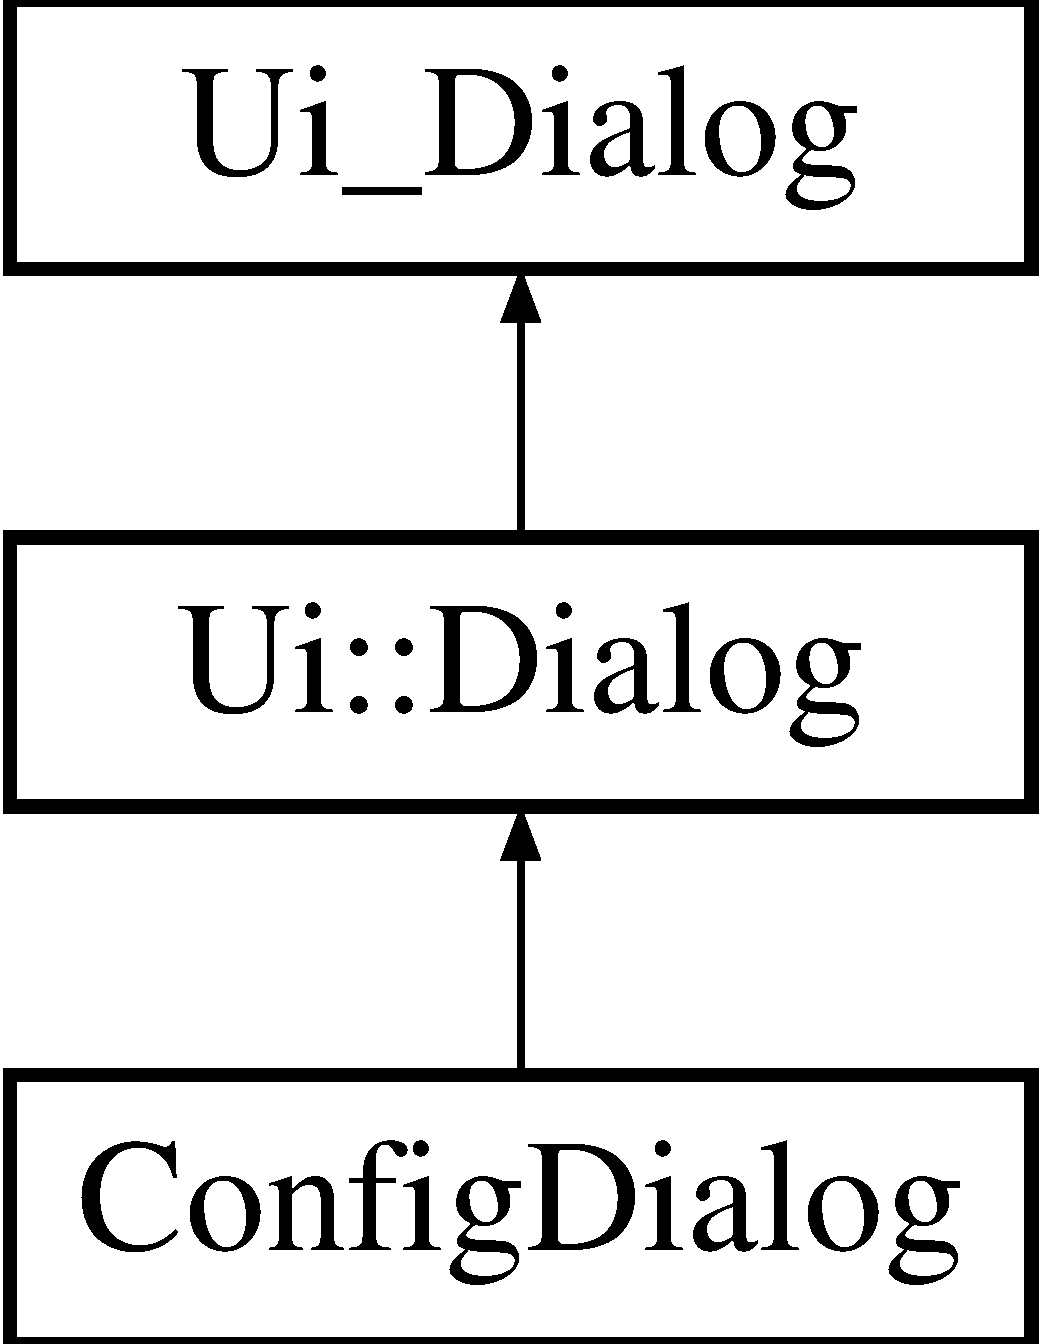
\includegraphics[height=3.000000cm]{class_config_dialog}
\end{center}
\end{figure}
\subsection*{Public Slots}
\begin{DoxyCompactItemize}
\item 
\hypertarget{class_config_dialog_ae2685db390eb8819ef04427010be9404}{
void {\bfseries renew} ()}
\label{class_config_dialog_ae2685db390eb8819ef04427010be9404}

\item 
\hypertarget{class_config_dialog_afacd2c7d5a0eb160c17f106008275054}{
void {\bfseries make\_\-config} ()}
\label{class_config_dialog_afacd2c7d5a0eb160c17f106008275054}

\end{DoxyCompactItemize}
\subsection*{Signals}
\begin{DoxyCompactItemize}
\item 
\hypertarget{class_config_dialog_ad515d4295b98da3b79bb604c71209dc7}{
void {\bfseries config\_\-ready} (\hyperlink{class_d_config}{DConfig} $\ast$config)}
\label{class_config_dialog_ad515d4295b98da3b79bb604c71209dc7}

\item 
\hypertarget{class_config_dialog_a228b0c52d645a86f9351a2df53f58279}{
void {\bfseries done} ()}
\label{class_config_dialog_a228b0c52d645a86f9351a2df53f58279}

\end{DoxyCompactItemize}
\subsection*{Public Member Functions}
\begin{DoxyCompactItemize}
\item 
\hypertarget{class_config_dialog_ad16df8ed2e55bd5cc55e3ef9040b8b93}{
{\bfseries ConfigDialog} (QWidget $\ast$parent=0)}
\label{class_config_dialog_ad16df8ed2e55bd5cc55e3ef9040b8b93}

\end{DoxyCompactItemize}
\subsection*{Public Attributes}
\begin{DoxyCompactItemize}
\item 
\hypertarget{class_config_dialog_a5ba7da0f4b32f7b2626d7a66631b4abb}{
\hyperlink{class_d_config}{DConfig} $\ast$ {\bfseries config}}
\label{class_config_dialog_a5ba7da0f4b32f7b2626d7a66631b4abb}

\end{DoxyCompactItemize}


The documentation for this class was generated from the following files:\begin{DoxyCompactItemize}
\item 
newConfigDialog/configdialog.h\item 
moc\_\-configdialog.cpp\item 
newConfigDialog/configdialog.cpp\end{DoxyCompactItemize}

\hypertarget{class_curve_data}{
\section{CurveData Class Reference}
\label{class_curve_data}\index{CurveData@{CurveData}}
}
\subsection*{Public Member Functions}
\begin{DoxyCompactItemize}
\item 
\hypertarget{class_curve_data_aa5a619af9980fa45612c98d438444b07}{
void {\bfseries append} (double $\ast$x, double $\ast$y, int count)}
\label{class_curve_data_aa5a619af9980fa45612c98d438444b07}

\item 
\hypertarget{class_curve_data_a6d3c0bbc2069cc39f265aa8e9ee5ad73}{
int {\bfseries count} () const }
\label{class_curve_data_a6d3c0bbc2069cc39f265aa8e9ee5ad73}

\item 
\hypertarget{class_curve_data_aa47747f11e103e908781800b278596d7}{
int {\bfseries size} () const }
\label{class_curve_data_aa47747f11e103e908781800b278596d7}

\item 
\hypertarget{class_curve_data_aeb1b65fe291fe72fa363640245383da4}{
const double $\ast$ {\bfseries x} () const }
\label{class_curve_data_aeb1b65fe291fe72fa363640245383da4}

\item 
\hypertarget{class_curve_data_a681ce130c86c62bcc1f6c488645f9b5b}{
const double $\ast$ {\bfseries y} () const }
\label{class_curve_data_a681ce130c86c62bcc1f6c488645f9b5b}

\item 
\hypertarget{class_curve_data_ae898810872a274a681ab60131ecf922b}{
void {\bfseries clear} ()}
\label{class_curve_data_ae898810872a274a681ab60131ecf922b}

\end{DoxyCompactItemize}


The documentation for this class was generated from the following files:\begin{DoxyCompactItemize}
\item 
includes/dcurve.h\item 
includes/dcurve.cpp\end{DoxyCompactItemize}

\hypertarget{class_d_config}{
\section{DConfig Class Reference}
\label{class_d_config}\index{DConfig@{DConfig}}
}
\subsection*{Public Attributes}
\begin{DoxyCompactItemize}
\item 
\hypertarget{class_d_config_aa2010c97b6b958035b554ae7eaaf5503}{
unsigned int {\bfseries table\_\-mod}}
\label{class_d_config_aa2010c97b6b958035b554ae7eaaf5503}

\item 
\hypertarget{class_d_config_a979590d630b81223da9f29a088961091}{
unsigned int {\bfseries chart\_\-mod}}
\label{class_d_config_a979590d630b81223da9f29a088961091}

\item 
\hypertarget{class_d_config_a0f4a14d70b0fd639b7e697031272fa5b}{
unsigned int {\bfseries measure\_\-num}}
\label{class_d_config_a0f4a14d70b0fd639b7e697031272fa5b}

\item 
\hypertarget{class_d_config_a8038ac83ad9d15884800e4e479e35c8b}{
unsigned int {\bfseries measure\_\-interval}}
\label{class_d_config_a8038ac83ad9d15884800e4e479e35c8b}

\item 
\hypertarget{class_d_config_a213a965c39046e3faa33a7d7cbdf9de1}{
QString {\bfseries filename}}
\label{class_d_config_a213a965c39046e3faa33a7d7cbdf9de1}

\item 
\hypertarget{class_d_config_a93f3cf9bf37010191cdacb01d6049af7}{
unsigned int {\bfseries mode}}
\label{class_d_config_a93f3cf9bf37010191cdacb01d6049af7}

\item 
\hypertarget{class_d_config_a3685b26c5b904e22b5cdc1a69e6efb9e}{
short unsigned int {\bfseries cycle\_\-mode}}
\label{class_d_config_a3685b26c5b904e22b5cdc1a69e6efb9e}

\item 
\hypertarget{class_d_config_a7ef6822f755e70db56a570b51e72f289}{
unsigned int {\bfseries cycle\_\-num}}
\label{class_d_config_a7ef6822f755e70db56a570b51e72f289}

\item 
\hypertarget{class_d_config_a740a1d70659efc7a3be4b3559ad621a1}{
unsigned int {\bfseries cycle\_\-interval}}
\label{class_d_config_a740a1d70659efc7a3be4b3559ad621a1}

\item 
\hypertarget{class_d_config_a595cbebf483fdb2d48c83d5ad2715258}{
unsigned int {\bfseries hour}}
\label{class_d_config_a595cbebf483fdb2d48c83d5ad2715258}

\item 
\hypertarget{class_d_config_aa9b1e1219f6fa3ab82a54bbcfd3cd6bd}{
unsigned int {\bfseries minute}}
\label{class_d_config_aa9b1e1219f6fa3ab82a54bbcfd3cd6bd}

\item 
\hypertarget{class_d_config_a3816f3dbc247f0f7e74ccd73bf399a91}{
unsigned int {\bfseries second}}
\label{class_d_config_a3816f3dbc247f0f7e74ccd73bf399a91}

\item 
\hypertarget{class_d_config_a55cfe8cf6f412f64d2a4656e7d5964a9}{
uint8\_\-t {\bfseries repeat}}
\label{class_d_config_a55cfe8cf6f412f64d2a4656e7d5964a9}

\item 
\hypertarget{class_d_config_a3bbf9ede5efa4c91a4aee84d36a575c7}{
unsigned int {\bfseries repeat\_\-interval}}
\label{class_d_config_a3bbf9ede5efa4c91a4aee84d36a575c7}

\item 
\hypertarget{class_d_config_a44e1595a55d4930358a573ecf13d0d11}{
QColor {\bfseries colors} \mbox{[}6\mbox{]}}
\label{class_d_config_a44e1595a55d4930358a573ecf13d0d11}

\end{DoxyCompactItemize}


The documentation for this class was generated from the following files:\begin{DoxyCompactItemize}
\item 
includes/dconfig.h\item 
includes/dconfig.cpp\end{DoxyCompactItemize}

\hypertarget{class_d_curve}{
\section{DCurve Class Reference}
\label{class_d_curve}\index{DCurve@{DCurve}}
}
\subsection*{Public Slots}
\begin{DoxyCompactItemize}
\item 
\hypertarget{class_d_curve_abf43db485286d4960afb1117d1b4fdb1}{
void {\bfseries accept\_\-data\_\-pack} (\hyperlink{struct_d_pack}{DPack} $\ast$pack)}
\label{class_d_curve_abf43db485286d4960afb1117d1b4fdb1}

\end{DoxyCompactItemize}
\subsection*{Signals}
\begin{DoxyCompactItemize}
\item 
\hypertarget{class_d_curve_aa6b8a386846b76a76fbcbc44e5830ee9}{
void {\bfseries pack\_\-accepted} ()}
\label{class_d_curve_aa6b8a386846b76a76fbcbc44e5830ee9}

\end{DoxyCompactItemize}
\subsection*{Public Member Functions}
\begin{DoxyCompactItemize}
\item 
\hypertarget{class_d_curve_a2f9fab43977d614e4e0e351e9f7e1917}{
{\bfseries DCurve} (QWidget $\ast$parent=0)}
\label{class_d_curve_a2f9fab43977d614e4e0e351e9f7e1917}

\item 
\hypertarget{class_d_curve_aeb642f1bae222064624dbb42e0c6eb03}{
void {\bfseries clear} ()}
\label{class_d_curve_aeb642f1bae222064624dbb42e0c6eb03}

\item 
\hypertarget{class_d_curve_a4fa1539a0d8d7dd5adfdb64f46f552c4}{
double {\bfseries getMaxX} ()}
\label{class_d_curve_a4fa1539a0d8d7dd5adfdb64f46f552c4}

\item 
\hypertarget{class_d_curve_a1604006983421bc479efe9e6383ebbf6}{
double {\bfseries getCurX} ()}
\label{class_d_curve_a1604006983421bc479efe9e6383ebbf6}

\item 
\hypertarget{class_d_curve_acf281464b139b0e65920430993c4e477}{
double {\bfseries getStepX} ()}
\label{class_d_curve_acf281464b139b0e65920430993c4e477}

\item 
\hypertarget{class_d_curve_a0c3999c4792840aed8a7979e3808612f}{
void {\bfseries setMaxX} (double x)}
\label{class_d_curve_a0c3999c4792840aed8a7979e3808612f}

\item 
\hypertarget{class_d_curve_a15b492423bc3f3e5bff4da4a6cf6db1b}{
void {\bfseries setCurX} (double x)}
\label{class_d_curve_a15b492423bc3f3e5bff4da4a6cf6db1b}

\item 
\hypertarget{class_d_curve_a8ff7ce13b6c2c132acd0a05c603620e0}{
void {\bfseries setStepX} (double x)}
\label{class_d_curve_a8ff7ce13b6c2c132acd0a05c603620e0}

\end{DoxyCompactItemize}
\subsection*{Public Attributes}
\begin{DoxyCompactItemize}
\item 
\hypertarget{class_d_curve_acc2db7ca766b9b5c2d9c6f7032397a03}{
QwtPlotCurve $\ast$ {\bfseries channel\_\-curve} \mbox{[}6\mbox{]}}
\label{class_d_curve_acc2db7ca766b9b5c2d9c6f7032397a03}

\item 
\hypertarget{class_d_curve_a5baf43c56f376816134a6142b507ec73}{
double {\bfseries curX}}
\label{class_d_curve_a5baf43c56f376816134a6142b507ec73}

\item 
\hypertarget{class_d_curve_a4f81003bc16287be2e4e66a3044a76d2}{
double {\bfseries maxX}}
\label{class_d_curve_a4f81003bc16287be2e4e66a3044a76d2}

\item 
\hypertarget{class_d_curve_a9bd8ccefa03ddc68cbfc03b1c3bb3a6e}{
double {\bfseries stepX}}
\label{class_d_curve_a9bd8ccefa03ddc68cbfc03b1c3bb3a6e}

\item 
\hypertarget{class_d_curve_a7b38ab86178c06b8196a296080238004}{
double {\bfseries curY}}
\label{class_d_curve_a7b38ab86178c06b8196a296080238004}

\item 
\hypertarget{class_d_curve_abb5763bcf75f0e9a7acff6f5034053ef}{
double $\ast$ {\bfseries bufX}}
\label{class_d_curve_abb5763bcf75f0e9a7acff6f5034053ef}

\item 
\hypertarget{class_d_curve_ab2bd801046ff512f1ee5b09ae1e90a04}{
double $\ast$ {\bfseries bufY}}
\label{class_d_curve_ab2bd801046ff512f1ee5b09ae1e90a04}

\end{DoxyCompactItemize}


The documentation for this class was generated from the following files:\begin{DoxyCompactItemize}
\item 
includes/dcurve.h\item 
includes/dcurve.cpp\item 
moc\_\-dcurve.cpp\end{DoxyCompactItemize}

\hypertarget{class_ui_1_1_dialog}{
\section{Ui::Dialog Class Reference}
\label{class_ui_1_1_dialog}\index{Ui::Dialog@{Ui::Dialog}}
}
Inheritance diagram for Ui::Dialog:\begin{figure}[H]
\begin{center}
\leavevmode
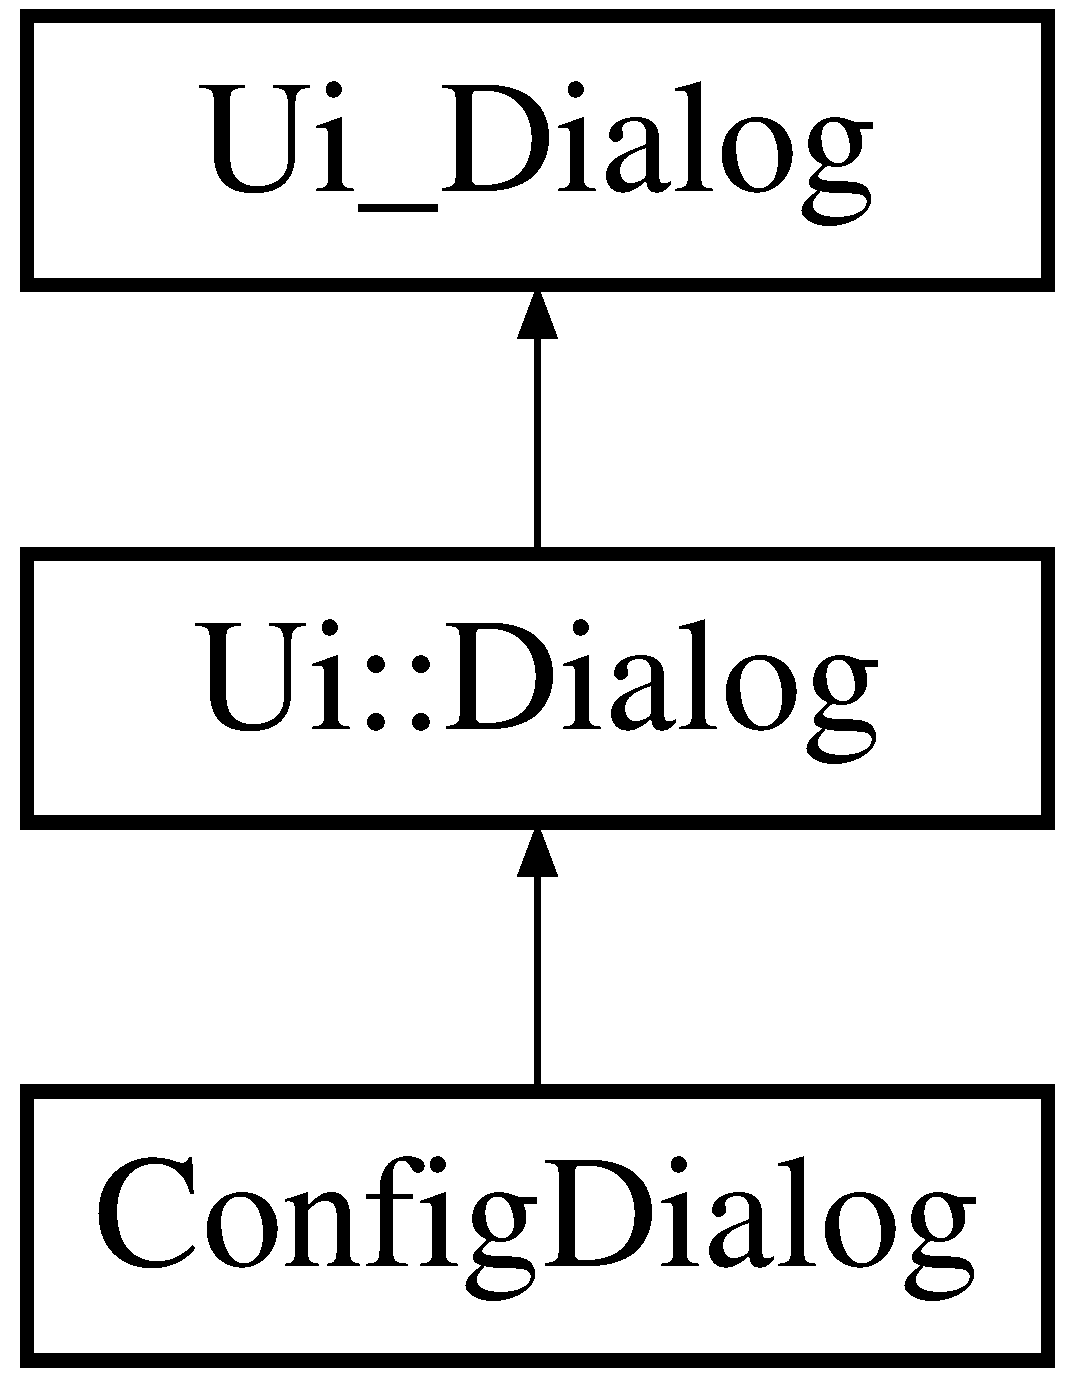
\includegraphics[height=3.000000cm]{class_ui_1_1_dialog}
\end{center}
\end{figure}


The documentation for this class was generated from the following file:\begin{DoxyCompactItemize}
\item 
ui\_\-configdialog.h\end{DoxyCompactItemize}

\hypertarget{struct_d_pack}{
\section{DPack Struct Reference}
\label{struct_d_pack}\index{DPack@{DPack}}
}
\subsection*{Public Attributes}
\begin{DoxyCompactItemize}
\item 
\hypertarget{struct_d_pack_afddb8374dde8ab256862ff6c01b5186c}{
QString {\bfseries data} \mbox{[}6\mbox{]}}
\label{struct_d_pack_afddb8374dde8ab256862ff6c01b5186c}

\end{DoxyCompactItemize}


The documentation for this struct was generated from the following file:\begin{DoxyCompactItemize}
\item 
includes/dpack.h\end{DoxyCompactItemize}

\hypertarget{class_d_saver}{
\section{DSaver Class Reference}
\label{class_d_saver}\index{DSaver@{DSaver}}
}
\subsection*{Public Slots}
\begin{DoxyCompactItemize}
\item 
\hypertarget{class_d_saver_a31c3409b66085c7465b364cd4f586a57}{
void {\bfseries accept\_\-string} (QString data)}
\label{class_d_saver_a31c3409b66085c7465b364cd4f586a57}

\item 
\hypertarget{class_d_saver_ac9e0c917baf8c95d5f9c670e35eb0374}{
void {\bfseries read\_\-string} ()}
\label{class_d_saver_ac9e0c917baf8c95d5f9c670e35eb0374}

\item 
\hypertarget{class_d_saver_a3120d68e1ce11a75001d492f4c8cf442}{
void {\bfseries set\_\-file\_\-name} (QString newName)}
\label{class_d_saver_a3120d68e1ce11a75001d492f4c8cf442}

\item 
\hypertarget{class_d_saver_a81e2d81811f5b8d08ca587aaae4f4645}{
void {\bfseries get\_\-file\_\-name} ()}
\label{class_d_saver_a81e2d81811f5b8d08ca587aaae4f4645}

\item 
\hypertarget{class_d_saver_a0a6d072bf09ceaec1495e390f963ad93}{
void {\bfseries accept\_\-data\_\-pack} (\hyperlink{struct_d_pack}{DPack} $\ast$pack)}
\label{class_d_saver_a0a6d072bf09ceaec1495e390f963ad93}

\item 
\hypertarget{class_d_saver_ae6a6f60800664717dd004299dadcc757}{
void {\bfseries read\_\-data\_\-pack} ()}
\label{class_d_saver_ae6a6f60800664717dd004299dadcc757}

\end{DoxyCompactItemize}
\subsection*{Signals}
\begin{DoxyCompactItemize}
\item 
\hypertarget{class_d_saver_ab785328826b004cb1b154a7452ce97a6}{
void {\bfseries saved} ()}
\label{class_d_saver_ab785328826b004cb1b154a7452ce97a6}

\item 
\hypertarget{class_d_saver_ac9fab0ee262742f0384df57631857a9f}{
void {\bfseries pack\_\-saved} ()}
\label{class_d_saver_ac9fab0ee262742f0384df57631857a9f}

\item 
\hypertarget{class_d_saver_ad828f0f14506fb5781f5a041fd378026}{
void {\bfseries name\_\-ready} ()}
\label{class_d_saver_ad828f0f14506fb5781f5a041fd378026}

\item 
\hypertarget{class_d_saver_a07788a99447703a36fdb1a78526b19b8}{
void {\bfseries string\_\-ready} (QString data)}
\label{class_d_saver_a07788a99447703a36fdb1a78526b19b8}

\item 
\hypertarget{class_d_saver_a3aab9fd72dbbd8629903276a00873b32}{
void {\bfseries pack\_\-ready} (\hyperlink{struct_d_pack}{DPack} $\ast$pack)}
\label{class_d_saver_a3aab9fd72dbbd8629903276a00873b32}

\end{DoxyCompactItemize}
\subsection*{Public Member Functions}
\begin{DoxyCompactItemize}
\item 
\hypertarget{class_d_saver_a1e80a72ab0d279c56774e426904ce98d}{
{\bfseries DSaver} (QWidget $\ast$parent=0)}
\label{class_d_saver_a1e80a72ab0d279c56774e426904ce98d}

\end{DoxyCompactItemize}


The documentation for this class was generated from the following files:\begin{DoxyCompactItemize}
\item 
includes/dsaver.h\item 
includes/dsaver.cpp\item 
moc\_\-dsaver.cpp\end{DoxyCompactItemize}

\hypertarget{class_d_thread}{
\section{DThread Class Reference}
\label{class_d_thread}\index{DThread@{DThread}}
}
\subsection*{Public Slots}
\begin{DoxyCompactItemize}
\item 
\hypertarget{class_d_thread_acb227b21c83bffd0120112fcf18d0713}{
void {\bfseries deliver\_\-data} (\hyperlink{struct_d_pack}{DPack} $\ast$pack)}
\label{class_d_thread_acb227b21c83bffd0120112fcf18d0713}

\item 
\hypertarget{class_d_thread_a740457d07f282ab8b6131252287bc14d}{
void {\bfseries set\_\-config} (\hyperlink{class_d_config}{DConfig} $\ast$cfg)}
\label{class_d_thread_a740457d07f282ab8b6131252287bc14d}

\item 
\hypertarget{class_d_thread_a8d8e1f1c17d6fbe700ff126d76d17187}{
void {\bfseries stop\_\-thread} ()}
\label{class_d_thread_a8d8e1f1c17d6fbe700ff126d76d17187}

\item 
\hypertarget{class_d_thread_acca0afdb09b445aa52408c86ce3e38a5}{
void {\bfseries start\_\-thread} ()}
\label{class_d_thread_acca0afdb09b445aa52408c86ce3e38a5}

\end{DoxyCompactItemize}
\subsection*{Signals}
\begin{DoxyCompactItemize}
\item 
\hypertarget{class_d_thread_a052faa4435bc9057a87c161b6bb570cf}{
void {\bfseries chart\_\-data} (\hyperlink{struct_d_pack}{DPack} $\ast$pack)}
\label{class_d_thread_a052faa4435bc9057a87c161b6bb570cf}

\item 
\hypertarget{class_d_thread_ace8013c8fbabb60e1ccb12eb630ec2fc}{
void {\bfseries text\_\-data} (\hyperlink{struct_d_pack}{DPack} $\ast$pack)}
\label{class_d_thread_ace8013c8fbabb60e1ccb12eb630ec2fc}

\item 
\hypertarget{class_d_thread_a5913dcefd646c4394c4421272059fd1e}{
void {\bfseries save\_\-data} (\hyperlink{struct_d_pack}{DPack} $\ast$pack)}
\label{class_d_thread_a5913dcefd646c4394c4421272059fd1e}

\item 
\hypertarget{class_d_thread_aad09f78cbf9b44a48697c405006527e3}{
void {\bfseries done} ()}
\label{class_d_thread_aad09f78cbf9b44a48697c405006527e3}

\item 
\hypertarget{class_d_thread_adfb0b72452e635f540c6a07ae0dad25c}{
void {\bfseries get\_\-config} (\hyperlink{class_d_config}{DConfig} $\ast$cfg)}
\label{class_d_thread_adfb0b72452e635f540c6a07ae0dad25c}

\item 
\hypertarget{class_d_thread_a35d637542b7766ea38f61768b824d1fd}{
void {\bfseries series\_\-start} ()}
\label{class_d_thread_a35d637542b7766ea38f61768b824d1fd}

\item 
\hypertarget{class_d_thread_aa70fd320d0eb6ef3b0da3b3338a9e07f}{
void {\bfseries series\_\-end} ()}
\label{class_d_thread_aa70fd320d0eb6ef3b0da3b3338a9e07f}

\end{DoxyCompactItemize}
\subsection*{Public Attributes}
\begin{DoxyCompactItemize}
\item 
\hypertarget{class_d_thread_af8950244842797b03785958c2ec66d1a}{
\hyperlink{class_d_config}{DConfig} $\ast$ {\bfseries config}}
\label{class_d_thread_af8950244842797b03785958c2ec66d1a}

\item 
\hypertarget{class_d_thread_ad8af957fb6500a12f65cf6847afbd205}{
\hyperlink{class_u_handler}{UHandler} $\ast$ {\bfseries device}}
\label{class_d_thread_ad8af957fb6500a12f65cf6847afbd205}

\end{DoxyCompactItemize}
\subsection*{Protected Member Functions}
\begin{DoxyCompactItemize}
\item 
\hypertarget{class_d_thread_a26a47da486d90f805cc39ccbf552e029}{
void {\bfseries run} ()}
\label{class_d_thread_a26a47da486d90f805cc39ccbf552e029}

\end{DoxyCompactItemize}


The documentation for this class was generated from the following files:\begin{DoxyCompactItemize}
\item 
includes/dthread.h\item 
includes/dthread.cpp\item 
moc\_\-dthread.cpp\end{DoxyCompactItemize}

\hypertarget{class_ui_1_1_main_window}{
\section{Ui::MainWindow Class Reference}
\label{class_ui_1_1_main_window}\index{Ui::MainWindow@{Ui::MainWindow}}
}
Inheritance diagram for Ui::MainWindow:\begin{figure}[H]
\begin{center}
\leavevmode
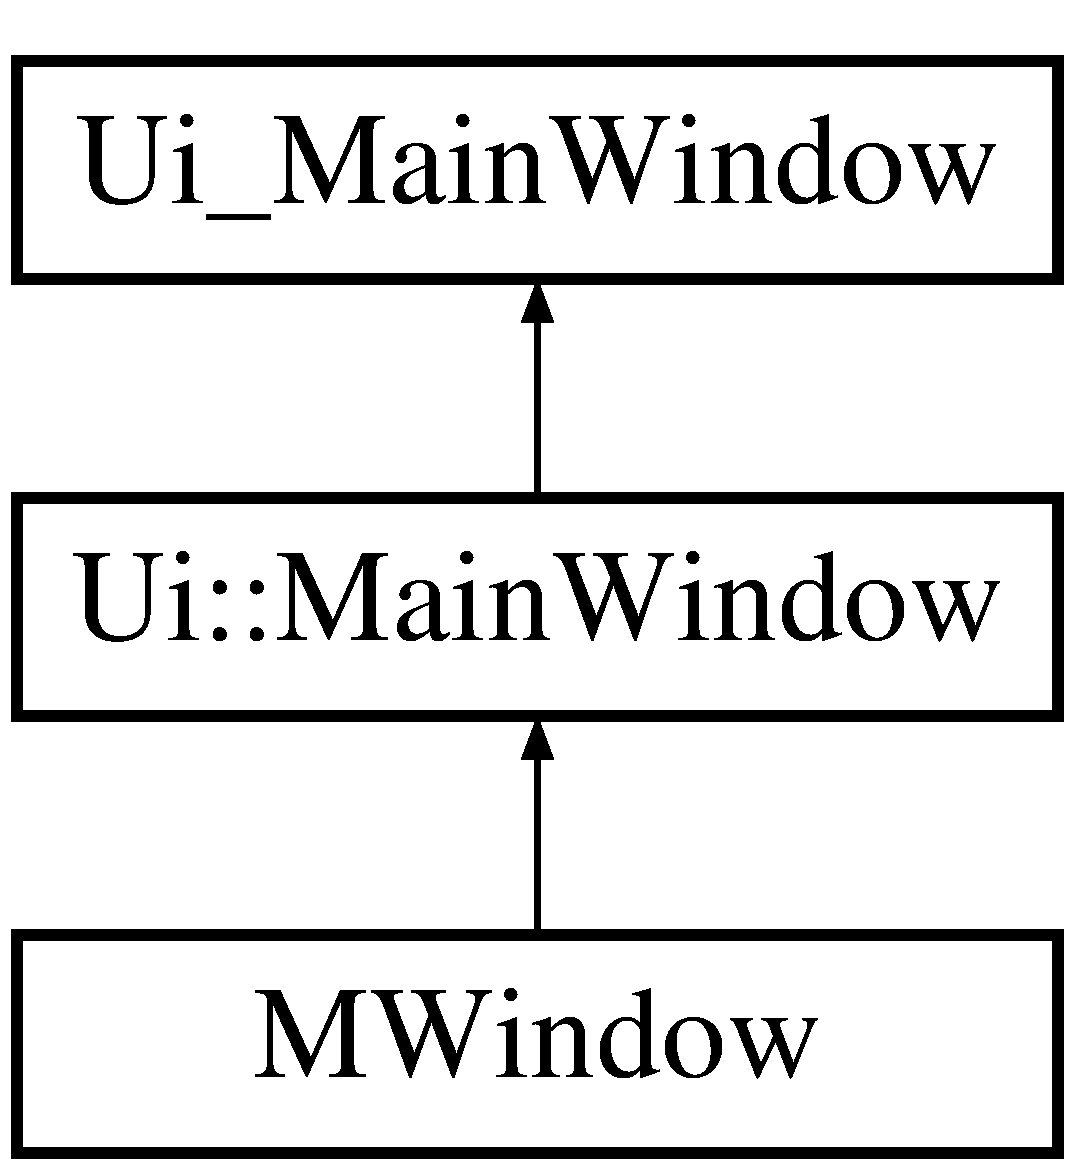
\includegraphics[height=3.000000cm]{class_ui_1_1_main_window}
\end{center}
\end{figure}


The documentation for this class was generated from the following file:\begin{DoxyCompactItemize}
\item 
ui\_\-mainwindow.h\end{DoxyCompactItemize}

\hypertarget{class_m_window}{
\section{MWindow Class Reference}
\label{class_m_window}\index{MWindow@{MWindow}}
}
Inheritance diagram for MWindow:\begin{figure}[H]
\begin{center}
\leavevmode
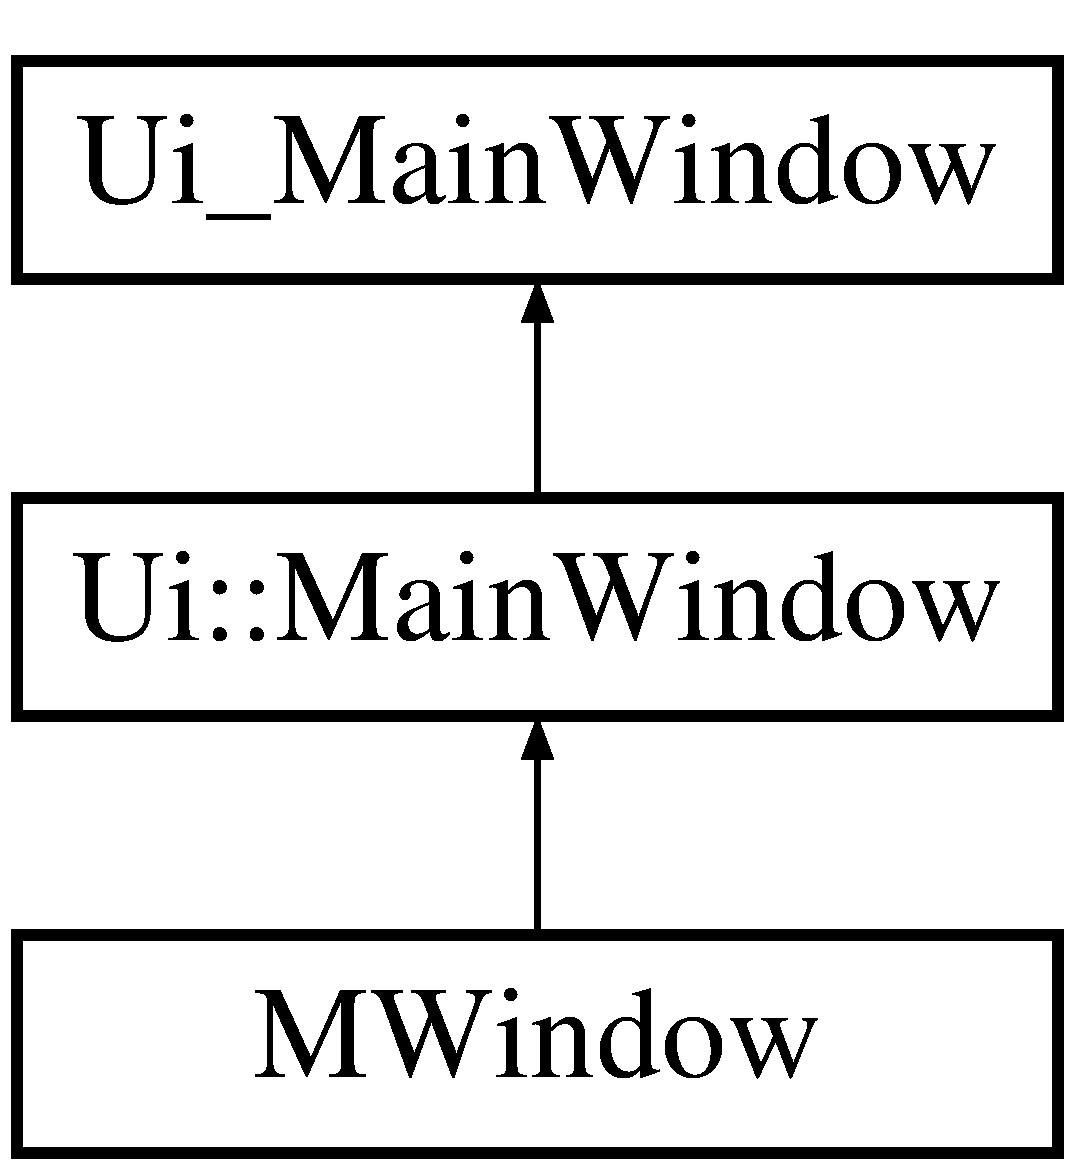
\includegraphics[height=3.000000cm]{class_m_window}
\end{center}
\end{figure}
\subsection*{Public Member Functions}
\begin{DoxyCompactItemize}
\item 
\hypertarget{class_m_window_abc4fd19ed9f1169de92322fcad7442fe}{
{\bfseries MWindow} (QWidget $\ast$parent=0)}
\label{class_m_window_abc4fd19ed9f1169de92322fcad7442fe}

\end{DoxyCompactItemize}


The documentation for this class was generated from the following files:\begin{DoxyCompactItemize}
\item 
mwindow.h\item 
mwindow.cpp\end{DoxyCompactItemize}

\hypertarget{class_ui_1_1process_dialog}{
\section{Ui::processDialog Class Reference}
\label{class_ui_1_1process_dialog}\index{Ui::processDialog@{Ui::processDialog}}
}
Inheritance diagram for Ui::processDialog:\begin{figure}[H]
\begin{center}
\leavevmode
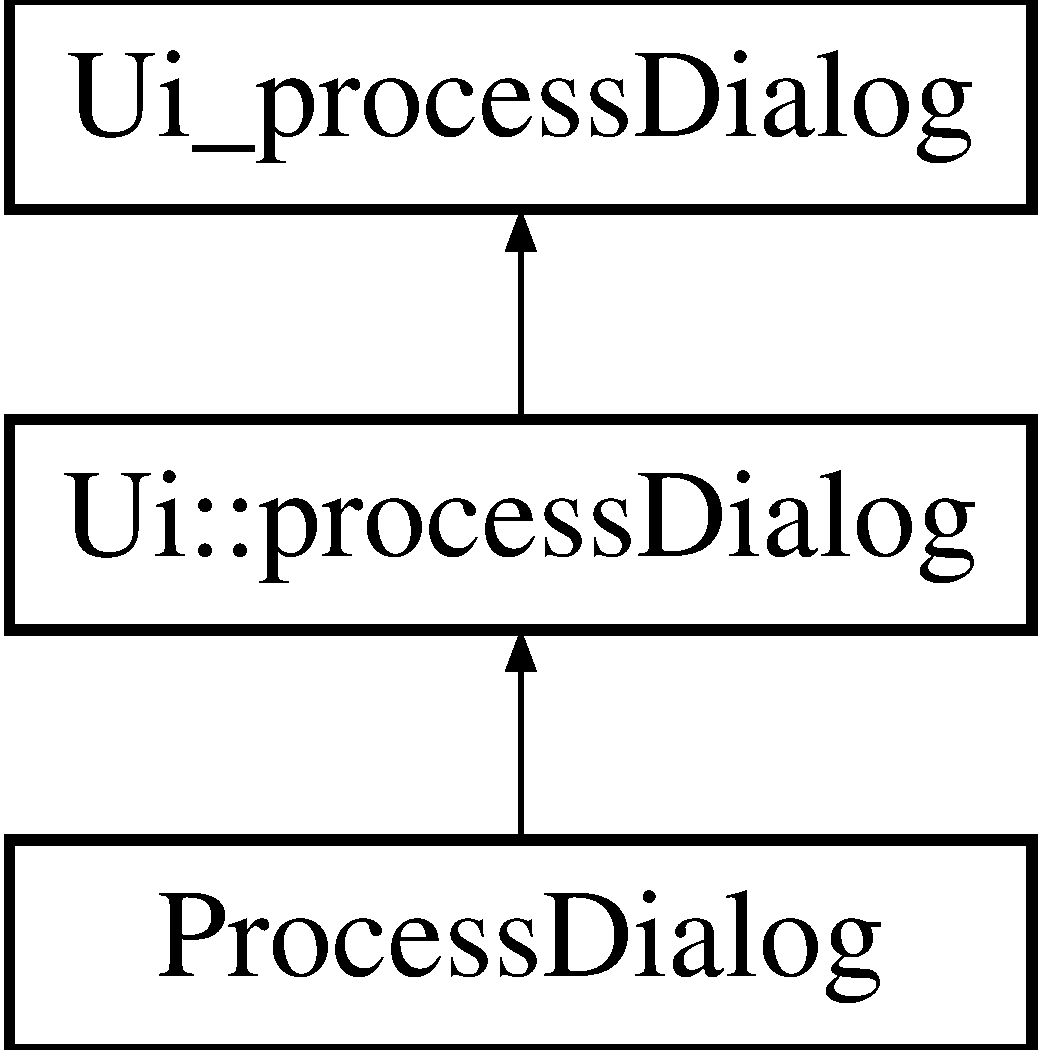
\includegraphics[height=3.000000cm]{class_ui_1_1process_dialog}
\end{center}
\end{figure}


The documentation for this class was generated from the following file:\begin{DoxyCompactItemize}
\item 
ui\_\-processdialog.h\end{DoxyCompactItemize}

\hypertarget{class_process_dialog}{
\section{ProcessDialog Class Reference}
\label{class_process_dialog}\index{ProcessDialog@{ProcessDialog}}
}
Inheritance diagram for ProcessDialog:\begin{figure}[H]
\begin{center}
\leavevmode
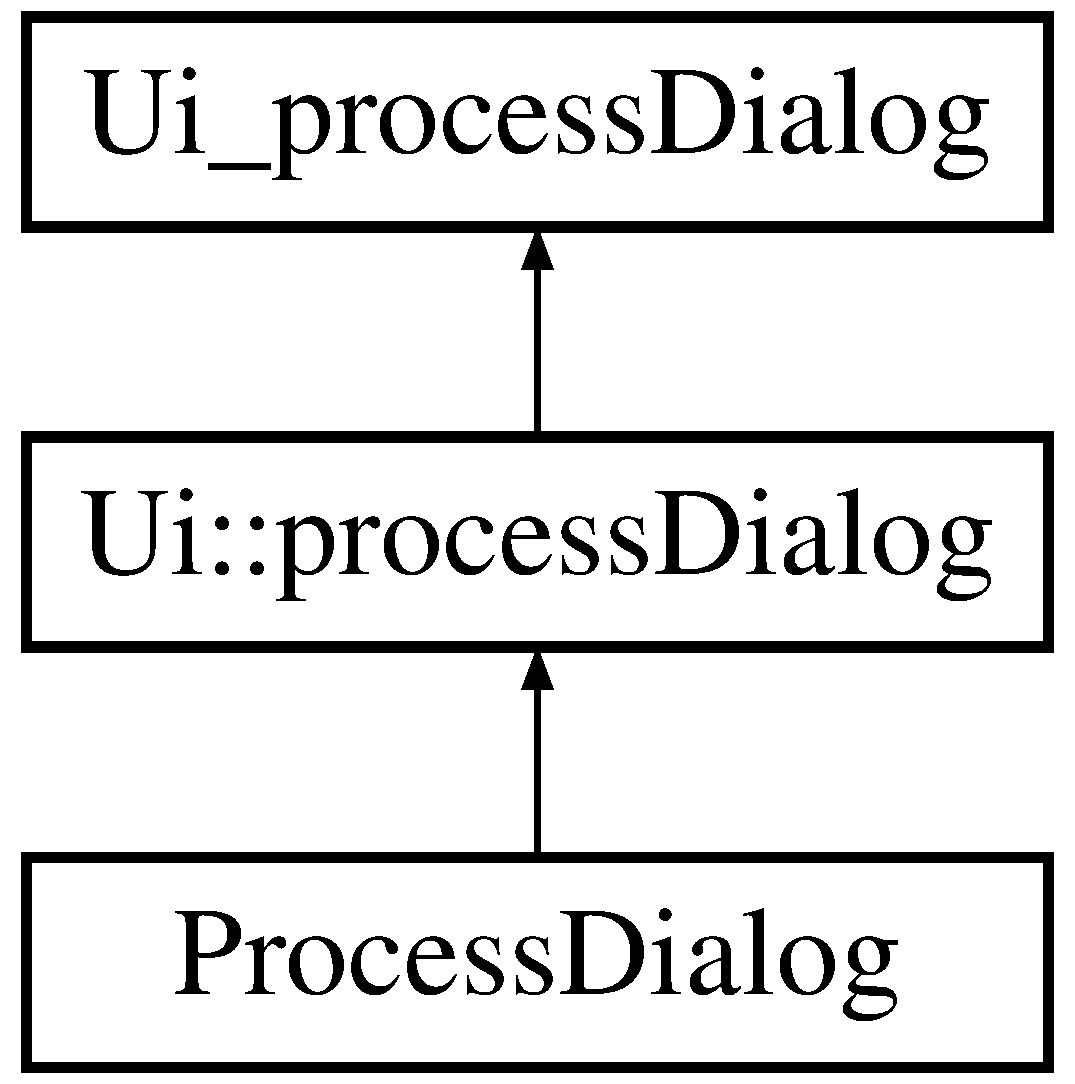
\includegraphics[height=3.000000cm]{class_process_dialog}
\end{center}
\end{figure}
\subsection*{Public Slots}
\begin{DoxyCompactItemize}
\item 
\hypertarget{class_process_dialog_a22a576af4d2abc52c268dca5d84198e6}{
void {\bfseries renew} ()}
\label{class_process_dialog_a22a576af4d2abc52c268dca5d84198e6}

\item 
\hypertarget{class_process_dialog_afbc030cfd27090f06a352c8b9b5c9dd4}{
void {\bfseries set\_\-config} (\hyperlink{class_d_config}{DConfig} $\ast$cfg)}
\label{class_process_dialog_afbc030cfd27090f06a352c8b9b5c9dd4}

\item 
\hypertarget{class_process_dialog_a862a117b87539153d8c31964fb0d9a13}{
void {\bfseries process\_\-pack} (\hyperlink{struct_d_pack}{DPack} $\ast$pack)}
\label{class_process_dialog_a862a117b87539153d8c31964fb0d9a13}

\item 
\hypertarget{class_process_dialog_aa18cc76fc46524dc707513feaefdb1d8}{
void {\bfseries start\_\-thread} ()}
\label{class_process_dialog_aa18cc76fc46524dc707513feaefdb1d8}

\end{DoxyCompactItemize}
\subsection*{Signals}
\begin{DoxyCompactItemize}
\item 
\hypertarget{class_process_dialog_aa701af7e78592295f979a21a57482e54}{
void {\bfseries stopped} ()}
\label{class_process_dialog_aa701af7e78592295f979a21a57482e54}

\item 
\hypertarget{class_process_dialog_aa76d8f8f2086b3b33752ebe2cd2f0926}{
void {\bfseries test\_\-data\_\-pack} (\hyperlink{struct_d_pack}{DPack} $\ast$pack)}
\label{class_process_dialog_aa76d8f8f2086b3b33752ebe2cd2f0926}

\end{DoxyCompactItemize}
\subsection*{Public Member Functions}
\begin{DoxyCompactItemize}
\item 
\hypertarget{class_process_dialog_a31e3e8798a5a9d16aa872c242c69ed82}{
{\bfseries ProcessDialog} (QWidget $\ast$parent=0)}
\label{class_process_dialog_a31e3e8798a5a9d16aa872c242c69ed82}

\end{DoxyCompactItemize}
\subsection*{Public Attributes}
\begin{DoxyCompactItemize}
\item 
\hypertarget{class_process_dialog_a157948d87442246dfd31f96e13964748}{
unsigned int {\bfseries zone\_\-length}}
\label{class_process_dialog_a157948d87442246dfd31f96e13964748}

\item 
\hypertarget{class_process_dialog_ac84aa88919bdd961f4590526e5249749}{
unsigned int {\bfseries start\_\-x}}
\label{class_process_dialog_ac84aa88919bdd961f4590526e5249749}

\item 
\hypertarget{class_process_dialog_a63d291adedc8c165137d50cc7a91af30}{
unsigned int {\bfseries end\_\-x}}
\label{class_process_dialog_a63d291adedc8c165137d50cc7a91af30}

\end{DoxyCompactItemize}


The documentation for this class was generated from the following files:\begin{DoxyCompactItemize}
\item 
processDialog/processdialog.h\item 
moc\_\-processdialog.cpp\item 
processDialog/processdialog.cpp\end{DoxyCompactItemize}

\hypertarget{class_u_handler}{
\section{UHandler Class Reference}
\label{class_u_handler}\index{UHandler@{UHandler}}
}
\subsection*{Public Slots}
\begin{DoxyCompactItemize}
\item 
\hypertarget{class_u_handler_a40e403e70909a4bb805bd97195ac92d7}{
void {\bfseries conversion\_\-request} ()}
\label{class_u_handler_a40e403e70909a4bb805bd97195ac92d7}

\item 
\hypertarget{class_u_handler_a3b5a9c04c309c144617781062e5cfabe}{
void {\bfseries set\_\-ccof} (double new\_\-ccof)}
\label{class_u_handler_a3b5a9c04c309c144617781062e5cfabe}

\end{DoxyCompactItemize}
\subsection*{Signals}
\begin{DoxyCompactItemize}
\item 
\hypertarget{class_u_handler_a742a8dab7c61c99f9435f598a7afa5fe}{
void {\bfseries data\_\-ready} ()}
\label{class_u_handler_a742a8dab7c61c99f9435f598a7afa5fe}

\item 
\hypertarget{class_u_handler_a968c8e73674c32ac0742609e30dcaed5}{
void {\bfseries data\_\-ready} (\hyperlink{struct_d_pack}{DPack} $\ast$datapack)}
\label{class_u_handler_a968c8e73674c32ac0742609e30dcaed5}

\item 
\hypertarget{class_u_handler_a67bbedf1977c775242c577aceaa5f60a}{
void {\bfseries deviceError} ()}
\label{class_u_handler_a67bbedf1977c775242c577aceaa5f60a}

\end{DoxyCompactItemize}
\subsection*{Public Member Functions}
\begin{DoxyCompactItemize}
\item 
\hypertarget{class_u_handler_af7d92c46f1bb7aec74f996518669d7d7}{
{\bfseries UHandler} (QWidget $\ast$parent=0)}
\label{class_u_handler_af7d92c46f1bb7aec74f996518669d7d7}

\end{DoxyCompactItemize}
\subsection*{Public Attributes}
\begin{DoxyCompactItemize}
\item 
\hypertarget{class_u_handler_aa7a1e60cd01885933bec8834ae3ae4e9}{
double {\bfseries ccof}}
\label{class_u_handler_aa7a1e60cd01885933bec8834ae3ae4e9}

\item 
\hypertarget{class_u_handler_ac89d9da8baa7fa903204e6a67d3a80bd}{
double {\bfseries results} \mbox{[}6\mbox{]}}
\label{class_u_handler_ac89d9da8baa7fa903204e6a67d3a80bd}

\item 
\hypertarget{class_u_handler_adce63833fe7060d728105361fec2d42f}{
\hyperlink{struct_d_pack}{DPack} {\bfseries pack}}
\label{class_u_handler_adce63833fe7060d728105361fec2d42f}

\end{DoxyCompactItemize}


The documentation for this class was generated from the following files:\begin{DoxyCompactItemize}
\item 
includes/uhandler.h\item 
includes/uhandler.cpp\item 
moc\_\-uhandler.cpp\end{DoxyCompactItemize}

\hypertarget{class_ui___dialog}{
\section{Ui\_\-Dialog Class Reference}
\label{class_ui___dialog}\index{Ui\_\-Dialog@{Ui\_\-Dialog}}
}
Inheritance diagram for Ui\_\-Dialog:\begin{figure}[H]
\begin{center}
\leavevmode
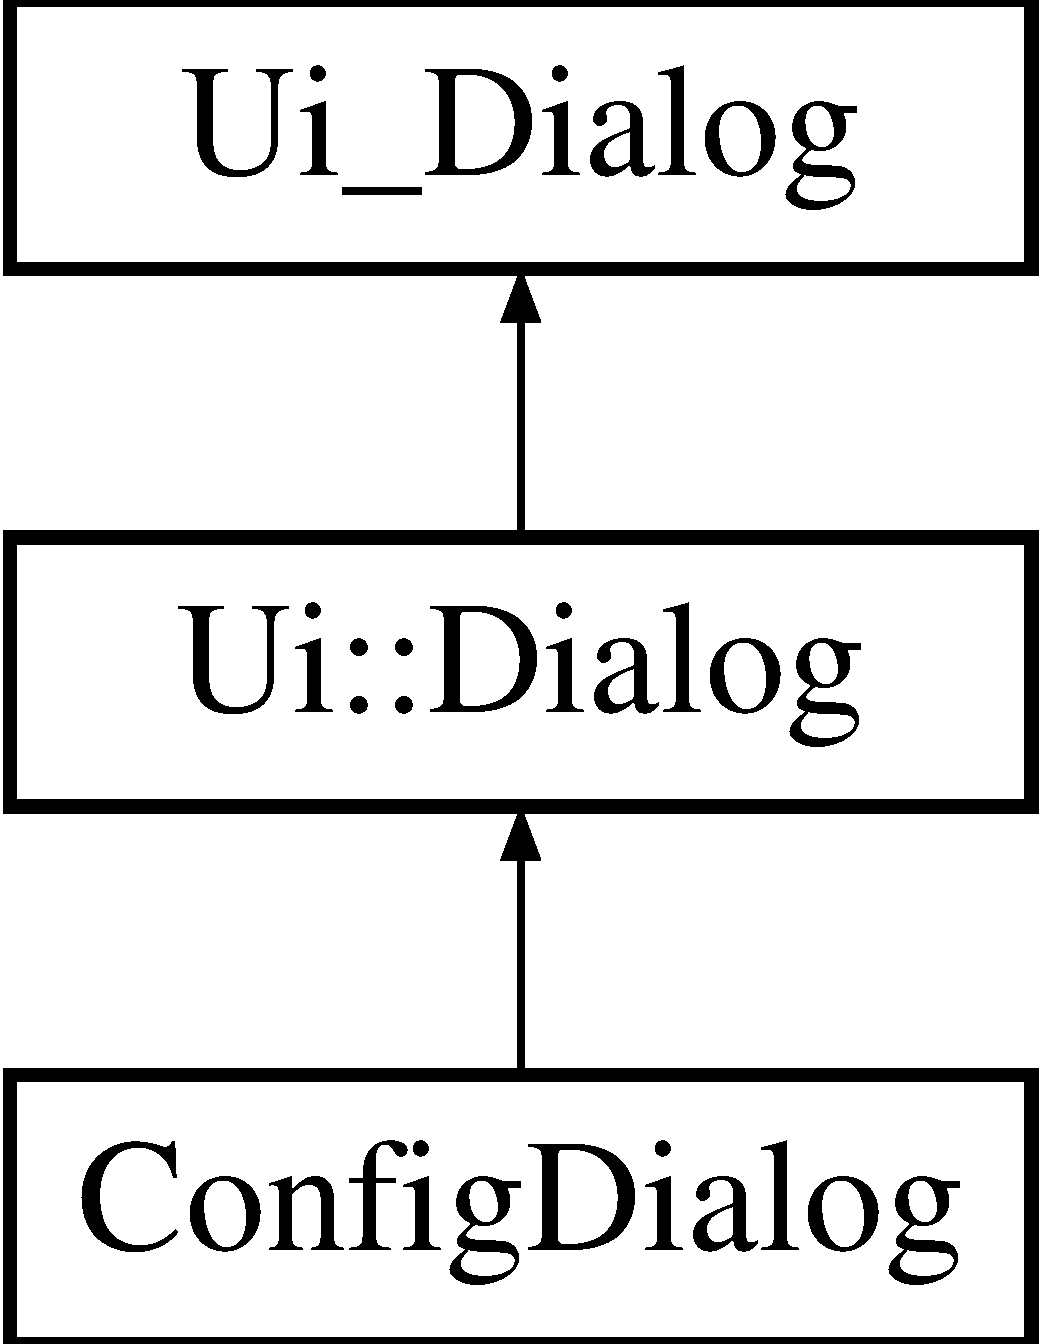
\includegraphics[height=3.000000cm]{class_ui___dialog}
\end{center}
\end{figure}
\subsection*{Public Member Functions}
\begin{DoxyCompactItemize}
\item 
\hypertarget{class_ui___dialog_a4f6a478c3ecdafabffb17b39cb26444a}{
void {\bfseries setupUi} (QDialog $\ast$Dialog)}
\label{class_ui___dialog_a4f6a478c3ecdafabffb17b39cb26444a}

\item 
\hypertarget{class_ui___dialog_afa0ccb6f716ca6178260522a193c250e}{
void {\bfseries retranslateUi} (QDialog $\ast$Dialog)}
\label{class_ui___dialog_afa0ccb6f716ca6178260522a193c250e}

\end{DoxyCompactItemize}
\subsection*{Public Attributes}
\begin{DoxyCompactItemize}
\item 
\hypertarget{class_ui___dialog_aeb2e76ae84a3a2c7943003b31fab3807}{
QWidget $\ast$ {\bfseries layoutWidget}}
\label{class_ui___dialog_aeb2e76ae84a3a2c7943003b31fab3807}

\item 
\hypertarget{class_ui___dialog_a937a02037ef2834dcab1b14df066bc6f}{
QHBoxLayout $\ast$ {\bfseries horizontalLayout\_\-11}}
\label{class_ui___dialog_a937a02037ef2834dcab1b14df066bc6f}

\item 
\hypertarget{class_ui___dialog_a5fa5f2b7f29d6d4bb0501e4348699871}{
QPushButton $\ast$ {\bfseries cancel\_\-button}}
\label{class_ui___dialog_a5fa5f2b7f29d6d4bb0501e4348699871}

\item 
\hypertarget{class_ui___dialog_a7f3697eebd238553ccbb5f716a16b00b}{
QPushButton $\ast$ {\bfseries proceed\_\-button}}
\label{class_ui___dialog_a7f3697eebd238553ccbb5f716a16b00b}

\item 
\hypertarget{class_ui___dialog_a9d40c4a031bcdc91ddc3500788f43a2c}{
QWidget $\ast$ {\bfseries layoutWidget1}}
\label{class_ui___dialog_a9d40c4a031bcdc91ddc3500788f43a2c}

\item 
\hypertarget{class_ui___dialog_aa5f63a5d3fdda1bfb39eaae06259f7de}{
QHBoxLayout $\ast$ {\bfseries horizontalLayout\_\-13}}
\label{class_ui___dialog_aa5f63a5d3fdda1bfb39eaae06259f7de}

\item 
\hypertarget{class_ui___dialog_a36913ded6b51b775719ffa4e49e955e2}{
QLabel $\ast$ {\bfseries table\_\-label1}}
\label{class_ui___dialog_a36913ded6b51b775719ffa4e49e955e2}

\item 
\hypertarget{class_ui___dialog_a505c0f026238a3e175f9e08e201713d7}{
QSpinBox $\ast$ {\bfseries table\_\-spin}}
\label{class_ui___dialog_a505c0f026238a3e175f9e08e201713d7}

\item 
\hypertarget{class_ui___dialog_a5ff04656bb940476c6880b7cca7a05a7}{
QLabel $\ast$ {\bfseries table\_\-label2}}
\label{class_ui___dialog_a5ff04656bb940476c6880b7cca7a05a7}

\item 
\hypertarget{class_ui___dialog_af959e1f33e58899284a9c05925bb4dc8}{
QWidget $\ast$ {\bfseries layoutWidget2}}
\label{class_ui___dialog_af959e1f33e58899284a9c05925bb4dc8}

\item 
\hypertarget{class_ui___dialog_a588f07833df3f10d10139816bf5adb3f}{
QHBoxLayout $\ast$ {\bfseries horizontalLayout\_\-14}}
\label{class_ui___dialog_a588f07833df3f10d10139816bf5adb3f}

\item 
\hypertarget{class_ui___dialog_a27c5acddae8a899b23ab77c154063a9d}{
QLabel $\ast$ {\bfseries graph\_\-label1}}
\label{class_ui___dialog_a27c5acddae8a899b23ab77c154063a9d}

\item 
\hypertarget{class_ui___dialog_a92bfcd2ffd3b08612fb8a7d4e444e4e3}{
QSpinBox $\ast$ {\bfseries chart\_\-spin}}
\label{class_ui___dialog_a92bfcd2ffd3b08612fb8a7d4e444e4e3}

\item 
\hypertarget{class_ui___dialog_a3dbee3c6468dda3601ae7f6daa2c09f0}{
QLabel $\ast$ {\bfseries graph\_\-label2}}
\label{class_ui___dialog_a3dbee3c6468dda3601ae7f6daa2c09f0}

\item 
\hypertarget{class_ui___dialog_a09b45474b3c768071a15b7876e520623}{
QWidget $\ast$ {\bfseries layoutWidget3}}
\label{class_ui___dialog_a09b45474b3c768071a15b7876e520623}

\item 
\hypertarget{class_ui___dialog_afa011080e484d395a5158edf7ae19c2a}{
QVBoxLayout $\ast$ {\bfseries verticalLayout\_\-5}}
\label{class_ui___dialog_afa011080e484d395a5158edf7ae19c2a}

\item 
\hypertarget{class_ui___dialog_a4ac89aafac432389fb3a29b85a9d5e77}{
QLabel $\ast$ {\bfseries measure\_\-label}}
\label{class_ui___dialog_a4ac89aafac432389fb3a29b85a9d5e77}

\item 
\hypertarget{class_ui___dialog_aba5f77de36ab458a482af58b2092275e}{
QHBoxLayout $\ast$ {\bfseries horizontalLayout\_\-16}}
\label{class_ui___dialog_aba5f77de36ab458a482af58b2092275e}

\item 
\hypertarget{class_ui___dialog_af6fefa91def76062d3cb8b1a7439abff}{
QSlider $\ast$ {\bfseries measure\_\-slider}}
\label{class_ui___dialog_af6fefa91def76062d3cb8b1a7439abff}

\item 
\hypertarget{class_ui___dialog_a897bd19f06897209fcd02eb807bf84b1}{
QSpinBox $\ast$ {\bfseries measure\_\-spin}}
\label{class_ui___dialog_a897bd19f06897209fcd02eb807bf84b1}

\item 
\hypertarget{class_ui___dialog_ae320f65502c05b3a83a0dcb891652eee}{
QLabel $\ast$ {\bfseries interval\_\-label}}
\label{class_ui___dialog_ae320f65502c05b3a83a0dcb891652eee}

\item 
\hypertarget{class_ui___dialog_ac44be1249046562e27691b3c0317782d}{
QHBoxLayout $\ast$ {\bfseries horizontalLayout\_\-17}}
\label{class_ui___dialog_ac44be1249046562e27691b3c0317782d}

\item 
\hypertarget{class_ui___dialog_a6441af2215d1b4082c3632a8b4576222}{
QSlider $\ast$ {\bfseries interval\_\-slider}}
\label{class_ui___dialog_a6441af2215d1b4082c3632a8b4576222}

\item 
\hypertarget{class_ui___dialog_ada0e5a6e464b6b76ef379c9ecc858762}{
QSpinBox $\ast$ {\bfseries interval\_\-spin}}
\label{class_ui___dialog_ada0e5a6e464b6b76ef379c9ecc858762}

\item 
\hypertarget{class_ui___dialog_add76f19fa17842298be5d3a84934c5c6}{
QWidget $\ast$ {\bfseries layoutWidget4}}
\label{class_ui___dialog_add76f19fa17842298be5d3a84934c5c6}

\item 
\hypertarget{class_ui___dialog_a4fb6d1c8d4780f0d513f4a48af4a2b10}{
QVBoxLayout $\ast$ {\bfseries verticalLayout\_\-2}}
\label{class_ui___dialog_a4fb6d1c8d4780f0d513f4a48af4a2b10}

\item 
\hypertarget{class_ui___dialog_ae84329827916f3da7d34ee7c16014936}{
QLabel $\ast$ {\bfseries filename\_\-label}}
\label{class_ui___dialog_ae84329827916f3da7d34ee7c16014936}

\item 
\hypertarget{class_ui___dialog_afdf33ddb6011cc0d723d43577fe1e39a}{
QHBoxLayout $\ast$ {\bfseries horizontalLayout\_\-15}}
\label{class_ui___dialog_afdf33ddb6011cc0d723d43577fe1e39a}

\item 
\hypertarget{class_ui___dialog_aaa85c8462692cbd2119d8a2038154263}{
QLineEdit $\ast$ {\bfseries filename\_\-edit}}
\label{class_ui___dialog_aaa85c8462692cbd2119d8a2038154263}

\item 
\hypertarget{class_ui___dialog_afb5aa711159788bfb5cd5837428eceab}{
QPushButton $\ast$ {\bfseries filename\_\-button}}
\label{class_ui___dialog_afb5aa711159788bfb5cd5837428eceab}

\item 
\hypertarget{class_ui___dialog_acea7e2baab6dcc329fd04b8edb4410f3}{
QGroupBox $\ast$ {\bfseries mode\_\-box}}
\label{class_ui___dialog_acea7e2baab6dcc329fd04b8edb4410f3}

\item 
\hypertarget{class_ui___dialog_a41336d41594e8776a81d095e8e4ffc61}{
QGridLayout $\ast$ {\bfseries gridLayout}}
\label{class_ui___dialog_a41336d41594e8776a81d095e8e4ffc61}

\item 
\hypertarget{class_ui___dialog_a02f973813b741621c5461918b3d9d4bb}{
QVBoxLayout $\ast$ {\bfseries verticalLayout}}
\label{class_ui___dialog_a02f973813b741621c5461918b3d9d4bb}

\item 
\hypertarget{class_ui___dialog_adb9e892e1f4ffbbdfdb607f5632a8893}{
QRadioButton $\ast$ {\bfseries single\_\-button}}
\label{class_ui___dialog_adb9e892e1f4ffbbdfdb607f5632a8893}

\item 
\hypertarget{class_ui___dialog_a02266ad6ec85260fd7ebda76ff582809}{
QRadioButton $\ast$ {\bfseries cycled\_\-button}}
\label{class_ui___dialog_a02266ad6ec85260fd7ebda76ff582809}

\item 
\hypertarget{class_ui___dialog_aaff883186ba4950da9d0bceb5819e6a6}{
QRadioButton $\ast$ {\bfseries scheduled\_\-button}}
\label{class_ui___dialog_aaff883186ba4950da9d0bceb5819e6a6}

\item 
\hypertarget{class_ui___dialog_a85edab9c7d1b081ff9ab106c9eb4a170}{
QGroupBox $\ast$ {\bfseries color\_\-box}}
\label{class_ui___dialog_a85edab9c7d1b081ff9ab106c9eb4a170}

\item 
\hypertarget{class_ui___dialog_af3de0f6556fd8c9d0aac09a2f90d92b9}{
QGridLayout $\ast$ {\bfseries gridLayout\_\-2}}
\label{class_ui___dialog_af3de0f6556fd8c9d0aac09a2f90d92b9}

\item 
\hypertarget{class_ui___dialog_ae66a1da203f045e33d71ed5abd46d2a1}{
QHBoxLayout $\ast$ {\bfseries horizontalLayout}}
\label{class_ui___dialog_ae66a1da203f045e33d71ed5abd46d2a1}

\item 
\hypertarget{class_ui___dialog_ae4a8ab2fa184ca5d64dc78d11e68825b}{
QLabel $\ast$ {\bfseries color\_\-label1}}
\label{class_ui___dialog_ae4a8ab2fa184ca5d64dc78d11e68825b}

\item 
\hypertarget{class_ui___dialog_a893bf5301fa97adbf73baa6efd8ce0cc}{
QPushButton $\ast$ {\bfseries color\_\-button1}}
\label{class_ui___dialog_a893bf5301fa97adbf73baa6efd8ce0cc}

\item 
\hypertarget{class_ui___dialog_a289b49bcdd28408efe2510f029535c2b}{
QHBoxLayout $\ast$ {\bfseries horizontalLayout\_\-2}}
\label{class_ui___dialog_a289b49bcdd28408efe2510f029535c2b}

\item 
\hypertarget{class_ui___dialog_ae1278eb2f6892786f9bc4a52da8d9972}{
QLabel $\ast$ {\bfseries color\_\-label2}}
\label{class_ui___dialog_ae1278eb2f6892786f9bc4a52da8d9972}

\item 
\hypertarget{class_ui___dialog_aa1e9fc847aeb79ce9de55bbe89902b18}{
QPushButton $\ast$ {\bfseries color\_\-button2}}
\label{class_ui___dialog_aa1e9fc847aeb79ce9de55bbe89902b18}

\item 
\hypertarget{class_ui___dialog_ab23bf4588fc8ad303dc922ef54138d15}{
QHBoxLayout $\ast$ {\bfseries horizontalLayout\_\-3}}
\label{class_ui___dialog_ab23bf4588fc8ad303dc922ef54138d15}

\item 
\hypertarget{class_ui___dialog_aae066f5be73df9ea14ee6bad8caa9395}{
QLabel $\ast$ {\bfseries color\_\-label3}}
\label{class_ui___dialog_aae066f5be73df9ea14ee6bad8caa9395}

\item 
\hypertarget{class_ui___dialog_afcdeb07facb9e6fbf0583e3d93059bd8}{
QPushButton $\ast$ {\bfseries color\_\-button3}}
\label{class_ui___dialog_afcdeb07facb9e6fbf0583e3d93059bd8}

\item 
\hypertarget{class_ui___dialog_ac3772f494bf164d526a04feff8314f96}{
QHBoxLayout $\ast$ {\bfseries horizontalLayout\_\-4}}
\label{class_ui___dialog_ac3772f494bf164d526a04feff8314f96}

\item 
\hypertarget{class_ui___dialog_ada959353b7a7e95c35bb4d8f8b7499df}{
QLabel $\ast$ {\bfseries color\_\-label4}}
\label{class_ui___dialog_ada959353b7a7e95c35bb4d8f8b7499df}

\item 
\hypertarget{class_ui___dialog_aa940462cd5f506fb74b20fdc2969c5e8}{
QPushButton $\ast$ {\bfseries color\_\-button4}}
\label{class_ui___dialog_aa940462cd5f506fb74b20fdc2969c5e8}

\item 
\hypertarget{class_ui___dialog_a47175a7aa879024aaa148e5c6c17d7fa}{
QHBoxLayout $\ast$ {\bfseries horizontalLayout\_\-5}}
\label{class_ui___dialog_a47175a7aa879024aaa148e5c6c17d7fa}

\item 
\hypertarget{class_ui___dialog_a5f877e437fe12237ed2466d27c133541}{
QLabel $\ast$ {\bfseries color\_\-label5}}
\label{class_ui___dialog_a5f877e437fe12237ed2466d27c133541}

\item 
\hypertarget{class_ui___dialog_a588e2e0b305a6e7afd5074b4ff933bcc}{
QPushButton $\ast$ {\bfseries color\_\-button5}}
\label{class_ui___dialog_a588e2e0b305a6e7afd5074b4ff933bcc}

\item 
\hypertarget{class_ui___dialog_a63eaa94aac456b7046c56286bf900694}{
QHBoxLayout $\ast$ {\bfseries horizontalLayout\_\-6}}
\label{class_ui___dialog_a63eaa94aac456b7046c56286bf900694}

\item 
\hypertarget{class_ui___dialog_a0e2fad831b2d03f0db9bbd3851b45545}{
QLabel $\ast$ {\bfseries color\_\-label6}}
\label{class_ui___dialog_a0e2fad831b2d03f0db9bbd3851b45545}

\item 
\hypertarget{class_ui___dialog_a0ad69be08b424e64c56d9159d73d47a5}{
QPushButton $\ast$ {\bfseries color\_\-button6}}
\label{class_ui___dialog_a0ad69be08b424e64c56d9159d73d47a5}

\item 
\hypertarget{class_ui___dialog_a765792d9269446951cd6126b95978baa}{
QWidget $\ast$ {\bfseries layoutWidget5}}
\label{class_ui___dialog_a765792d9269446951cd6126b95978baa}

\item 
\hypertarget{class_ui___dialog_a5ea05598d639698eabf0cbc00b1f0180}{
QVBoxLayout $\ast$ {\bfseries verticalLayout\_\-4}}
\label{class_ui___dialog_a5ea05598d639698eabf0cbc00b1f0180}

\item 
\hypertarget{class_ui___dialog_a6493a4b5d1d60438e2e6d8da6084a7f7}{
QLabel $\ast$ {\bfseries series\_\-time\_\-label}}
\label{class_ui___dialog_a6493a4b5d1d60438e2e6d8da6084a7f7}

\item 
\hypertarget{class_ui___dialog_aa29901501eb3d813512e5909ee046593}{
QLineEdit $\ast$ {\bfseries series\_\-time\_\-edit}}
\label{class_ui___dialog_aa29901501eb3d813512e5909ee046593}

\item 
\hypertarget{class_ui___dialog_aa25a19014320de47e6069229ec548314}{
QWidget $\ast$ {\bfseries layoutWidget6}}
\label{class_ui___dialog_aa25a19014320de47e6069229ec548314}

\item 
\hypertarget{class_ui___dialog_a462b148b6c1e7eaba6440e0dab6b1fd3}{
QHBoxLayout $\ast$ {\bfseries horizontalLayout\_\-18}}
\label{class_ui___dialog_a462b148b6c1e7eaba6440e0dab6b1fd3}

\item 
\hypertarget{class_ui___dialog_a88231f085e6e959b243f63a9198e9983}{
QGroupBox $\ast$ {\bfseries schedule\_\-box}}
\label{class_ui___dialog_a88231f085e6e959b243f63a9198e9983}

\item 
\hypertarget{class_ui___dialog_a607cdeee5a14c32de985d3909365f033}{
QGridLayout $\ast$ {\bfseries gridLayout\_\-4}}
\label{class_ui___dialog_a607cdeee5a14c32de985d3909365f033}

\item 
\hypertarget{class_ui___dialog_acd165ec013acc890cb290ce16b9563f6}{
QVBoxLayout $\ast$ {\bfseries verticalLayout\_\-3}}
\label{class_ui___dialog_acd165ec013acc890cb290ce16b9563f6}

\item 
\hypertarget{class_ui___dialog_a3789ef0751d9736778a489d90d9a4272}{
QLabel $\ast$ {\bfseries schedule\_\-label}}
\label{class_ui___dialog_a3789ef0751d9736778a489d90d9a4272}

\item 
\hypertarget{class_ui___dialog_af48abfeb780fc4fdf2129c6c9a05984e}{
QHBoxLayout $\ast$ {\bfseries horizontalLayout\_\-8}}
\label{class_ui___dialog_af48abfeb780fc4fdf2129c6c9a05984e}

\item 
\hypertarget{class_ui___dialog_a2c65e7ef9bf552e69d42c94c17266506}{
QSpinBox $\ast$ {\bfseries hours\_\-box}}
\label{class_ui___dialog_a2c65e7ef9bf552e69d42c94c17266506}

\item 
\hypertarget{class_ui___dialog_a7d2f3eda798178a4fa9a443d90acbee7}{
QLabel $\ast$ {\bfseries hours\_\-label}}
\label{class_ui___dialog_a7d2f3eda798178a4fa9a443d90acbee7}

\item 
\hypertarget{class_ui___dialog_a03ce64accc7b2dbd50c7b7f6e9ddd2b7}{
QSpinBox $\ast$ {\bfseries minutes\_\-box}}
\label{class_ui___dialog_a03ce64accc7b2dbd50c7b7f6e9ddd2b7}

\item 
\hypertarget{class_ui___dialog_adfd82d3f26f58359dce559a7ac749c47}{
QLabel $\ast$ {\bfseries minutes\_\-label}}
\label{class_ui___dialog_adfd82d3f26f58359dce559a7ac749c47}

\item 
\hypertarget{class_ui___dialog_af248d8c93e202b513f89a5f1d512467f}{
QSpinBox $\ast$ {\bfseries seconds\_\-box}}
\label{class_ui___dialog_af248d8c93e202b513f89a5f1d512467f}

\item 
\hypertarget{class_ui___dialog_aa24e2efaa316c1309ff4dbca49d38aad}{
QLabel $\ast$ {\bfseries seconds\_\-label}}
\label{class_ui___dialog_aa24e2efaa316c1309ff4dbca49d38aad}

\item 
\hypertarget{class_ui___dialog_a501687e996bc322aaeb0ad55909ac7d9}{
QHBoxLayout $\ast$ {\bfseries horizontalLayout\_\-9}}
\label{class_ui___dialog_a501687e996bc322aaeb0ad55909ac7d9}

\item 
\hypertarget{class_ui___dialog_aec0cf1628383935e9b8003e9d65da3f6}{
QCheckBox $\ast$ {\bfseries sd\_\-box}}
\label{class_ui___dialog_aec0cf1628383935e9b8003e9d65da3f6}

\item 
\hypertarget{class_ui___dialog_a8c81129e26e3da217bbb9220588a2e6d}{
QCheckBox $\ast$ {\bfseries mn\_\-box}}
\label{class_ui___dialog_a8c81129e26e3da217bbb9220588a2e6d}

\item 
\hypertarget{class_ui___dialog_ad1d1ee845fd267d3caa799082efdc639}{
QCheckBox $\ast$ {\bfseries tue\_\-box}}
\label{class_ui___dialog_ad1d1ee845fd267d3caa799082efdc639}

\item 
\hypertarget{class_ui___dialog_a9aba2fb39c731818127fba8996826c24}{
QCheckBox $\ast$ {\bfseries wd\_\-box}}
\label{class_ui___dialog_a9aba2fb39c731818127fba8996826c24}

\item 
\hypertarget{class_ui___dialog_a4bb59b2c7c5cc675828f853348cf81b4}{
QHBoxLayout $\ast$ {\bfseries horizontalLayout\_\-10}}
\label{class_ui___dialog_a4bb59b2c7c5cc675828f853348cf81b4}

\item 
\hypertarget{class_ui___dialog_a43f82baf51e4bd06c10bde0174a3be4d}{
QCheckBox $\ast$ {\bfseries th\_\-box}}
\label{class_ui___dialog_a43f82baf51e4bd06c10bde0174a3be4d}

\item 
\hypertarget{class_ui___dialog_a6249084e503475fe9c0542fbd054af60}{
QCheckBox $\ast$ {\bfseries fr\_\-box}}
\label{class_ui___dialog_a6249084e503475fe9c0542fbd054af60}

\item 
\hypertarget{class_ui___dialog_a9cf7c3d10db508f957b64b65dcc29f75}{
QCheckBox $\ast$ {\bfseries sat\_\-box}}
\label{class_ui___dialog_a9cf7c3d10db508f957b64b65dcc29f75}

\item 
\hypertarget{class_ui___dialog_afc1d1f7e78c2b36ca4fe66cd1c489dd8}{
QCheckBox $\ast$ {\bfseries schedule\_\-repeat}}
\label{class_ui___dialog_afc1d1f7e78c2b36ca4fe66cd1c489dd8}

\item 
\hypertarget{class_ui___dialog_ab0aa9cf0408f97f51f4277d0a0077b23}{
QGroupBox $\ast$ {\bfseries cycle\_\-box}}
\label{class_ui___dialog_ab0aa9cf0408f97f51f4277d0a0077b23}

\item 
\hypertarget{class_ui___dialog_a95e4393e872e5101ebfc05e5e5cd182f}{
QGridLayout $\ast$ {\bfseries gridLayout\_\-3}}
\label{class_ui___dialog_a95e4393e872e5101ebfc05e5e5cd182f}

\item 
\hypertarget{class_ui___dialog_acecca3df0d4bc0c913da56f2b7acee32}{
QHBoxLayout $\ast$ {\bfseries horizontalLayout\_\-7}}
\label{class_ui___dialog_acecca3df0d4bc0c913da56f2b7acee32}

\item 
\hypertarget{class_ui___dialog_a6b0d865e7e952ba13465d386ace85cc4}{
QCheckBox $\ast$ {\bfseries cycle\_\-infinite}}
\label{class_ui___dialog_a6b0d865e7e952ba13465d386ace85cc4}

\item 
\hypertarget{class_ui___dialog_aed1358d8a6fb592ee96c17cc2e77d2eb}{
QLabel $\ast$ {\bfseries cycle\_\-number\_\-label}}
\label{class_ui___dialog_aed1358d8a6fb592ee96c17cc2e77d2eb}

\item 
\hypertarget{class_ui___dialog_aff7e7545fada626eee557c7061bb37ef}{
QHBoxLayout $\ast$ {\bfseries horizontalLayout\_\-12}}
\label{class_ui___dialog_aff7e7545fada626eee557c7061bb37ef}

\item 
\hypertarget{class_ui___dialog_a24355e2474039f1b7d2ef294acde0434}{
QSlider $\ast$ {\bfseries cycle\_\-number\_\-slider}}
\label{class_ui___dialog_a24355e2474039f1b7d2ef294acde0434}

\item 
\hypertarget{class_ui___dialog_a0be189bc5eb8101f29b338b860879102}{
QSpinBox $\ast$ {\bfseries cycle\_\-number\_\-spin}}
\label{class_ui___dialog_a0be189bc5eb8101f29b338b860879102}

\item 
\hypertarget{class_ui___dialog_a105ac15a30b525f4d74b483428c13eb6}{
QLabel $\ast$ {\bfseries cycle\_\-repeat\_\-label}}
\label{class_ui___dialog_a105ac15a30b525f4d74b483428c13eb6}

\item 
\hypertarget{class_ui___dialog_a45848d5ddee2a1fec7b25bd305f0b2a8}{
QVBoxLayout $\ast$ {\bfseries verticalLayout\_\-6}}
\label{class_ui___dialog_a45848d5ddee2a1fec7b25bd305f0b2a8}

\item 
\hypertarget{class_ui___dialog_ad76be9e0352482970223593beb77ce5c}{
QSlider $\ast$ {\bfseries cycle\_\-interval\_\-slider}}
\label{class_ui___dialog_ad76be9e0352482970223593beb77ce5c}

\item 
\hypertarget{class_ui___dialog_a48ce2da4a2452ed43632629417fad134}{
QSpinBox $\ast$ {\bfseries cycle\_\-interval\_\-spin}}
\label{class_ui___dialog_a48ce2da4a2452ed43632629417fad134}

\end{DoxyCompactItemize}


The documentation for this class was generated from the following file:\begin{DoxyCompactItemize}
\item 
ui\_\-configdialog.h\end{DoxyCompactItemize}

\hypertarget{class_ui___main_window}{
\section{Ui\_\-MainWindow Class Reference}
\label{class_ui___main_window}\index{Ui\_\-MainWindow@{Ui\_\-MainWindow}}
}
Inheritance diagram for Ui\_\-MainWindow:\begin{figure}[H]
\begin{center}
\leavevmode
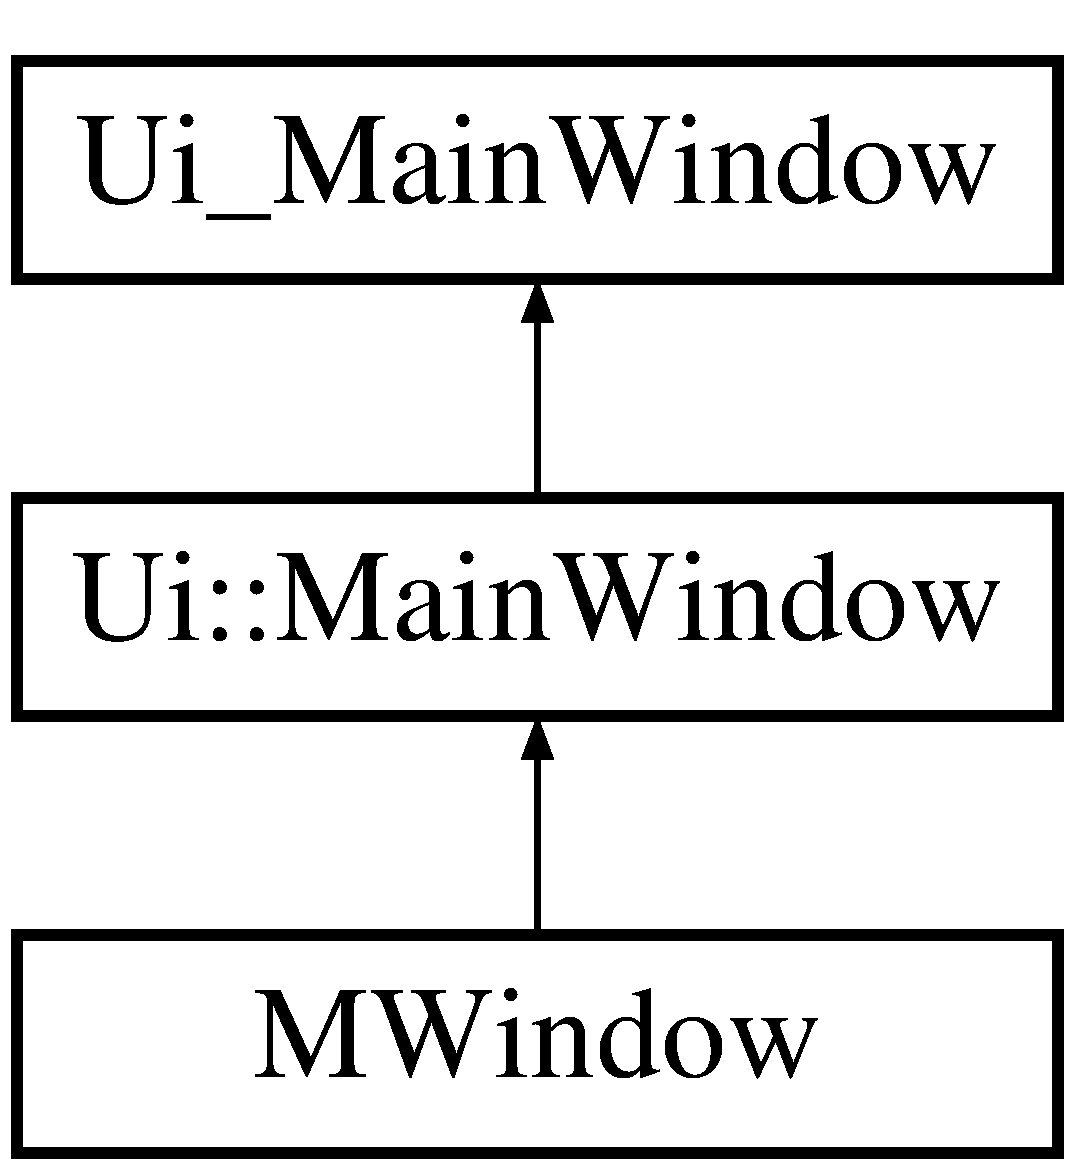
\includegraphics[height=3.000000cm]{class_ui___main_window}
\end{center}
\end{figure}
\subsection*{Public Member Functions}
\begin{DoxyCompactItemize}
\item 
\hypertarget{class_ui___main_window_acf4a0872c4c77d8f43a2ec66ed849b58}{
void {\bfseries setupUi} (QMainWindow $\ast$MainWindow)}
\label{class_ui___main_window_acf4a0872c4c77d8f43a2ec66ed849b58}

\item 
\hypertarget{class_ui___main_window_a097dd160c3534a204904cb374412c618}{
void {\bfseries retranslateUi} (QMainWindow $\ast$MainWindow)}
\label{class_ui___main_window_a097dd160c3534a204904cb374412c618}

\end{DoxyCompactItemize}
\subsection*{Public Attributes}
\begin{DoxyCompactItemize}
\item 
\hypertarget{class_ui___main_window_a5b65436e6cc259d5586eb6e309b612e4}{
QAction $\ast$ {\bfseries actionSettings}}
\label{class_ui___main_window_a5b65436e6cc259d5586eb6e309b612e4}

\item 
\hypertarget{class_ui___main_window_a5f16414653ef549d2ee14b730946a797}{
QAction $\ast$ {\bfseries actionPlugins}}
\label{class_ui___main_window_a5f16414653ef549d2ee14b730946a797}

\item 
\hypertarget{class_ui___main_window_ae8370529640da51b50cd1fb5be677c02}{
QAction $\ast$ {\bfseries actionExit}}
\label{class_ui___main_window_ae8370529640da51b50cd1fb5be677c02}

\item 
\hypertarget{class_ui___main_window_abdf2b43167c2cd0d3405f90b8c30e934}{
QAction $\ast$ {\bfseries actionAbout}}
\label{class_ui___main_window_abdf2b43167c2cd0d3405f90b8c30e934}

\item 
\hypertarget{class_ui___main_window_a356f1cf3ebda15f1fac59467ee081b74}{
QWidget $\ast$ {\bfseries centralwidget}}
\label{class_ui___main_window_a356f1cf3ebda15f1fac59467ee081b74}

\item 
\hypertarget{class_ui___main_window_a6b2a0c5f7e8ff2a87134908dd770d2d2}{
QGridLayout $\ast$ {\bfseries gridLayout\_\-2}}
\label{class_ui___main_window_a6b2a0c5f7e8ff2a87134908dd770d2d2}

\item 
\hypertarget{class_ui___main_window_a525ed3c5fe0784ac502ee222fba4e205}{
QGridLayout $\ast$ {\bfseries gridLayout}}
\label{class_ui___main_window_a525ed3c5fe0784ac502ee222fba4e205}

\item 
\hypertarget{class_ui___main_window_a5b1dcfe4176a82a548cf76fff38e0bf2}{
QPushButton $\ast$ {\bfseries newButton}}
\label{class_ui___main_window_a5b1dcfe4176a82a548cf76fff38e0bf2}

\item 
\hypertarget{class_ui___main_window_a51a49c117798bbe31cee18f0d0dc1237}{
QPushButton $\ast$ {\bfseries closeButton}}
\label{class_ui___main_window_a51a49c117798bbe31cee18f0d0dc1237}

\item 
\hypertarget{class_ui___main_window_ad25d7acd430daf05ee3459c1cba9af69}{
QPushButton $\ast$ {\bfseries aboutButton}}
\label{class_ui___main_window_ad25d7acd430daf05ee3459c1cba9af69}

\item 
\hypertarget{class_ui___main_window_adf43d9a67adaec750aaa956b5e082f09}{
QMenuBar $\ast$ {\bfseries menubar}}
\label{class_ui___main_window_adf43d9a67adaec750aaa956b5e082f09}

\item 
\hypertarget{class_ui___main_window_a6d7bbbef44e207ee15e5a623171033a2}{
QMenu $\ast$ {\bfseries menuMenu}}
\label{class_ui___main_window_a6d7bbbef44e207ee15e5a623171033a2}

\item 
\hypertarget{class_ui___main_window_a1687cceb1e2787aa1f83e50433943a91}{
QStatusBar $\ast$ {\bfseries statusbar}}
\label{class_ui___main_window_a1687cceb1e2787aa1f83e50433943a91}

\end{DoxyCompactItemize}


The documentation for this class was generated from the following file:\begin{DoxyCompactItemize}
\item 
ui\_\-mainwindow.h\end{DoxyCompactItemize}

\hypertarget{class_ui__process_dialog}{
\section{Ui\_\-processDialog Class Reference}
\label{class_ui__process_dialog}\index{Ui\_\-processDialog@{Ui\_\-processDialog}}
}
Inheritance diagram for Ui\_\-processDialog:\begin{figure}[H]
\begin{center}
\leavevmode
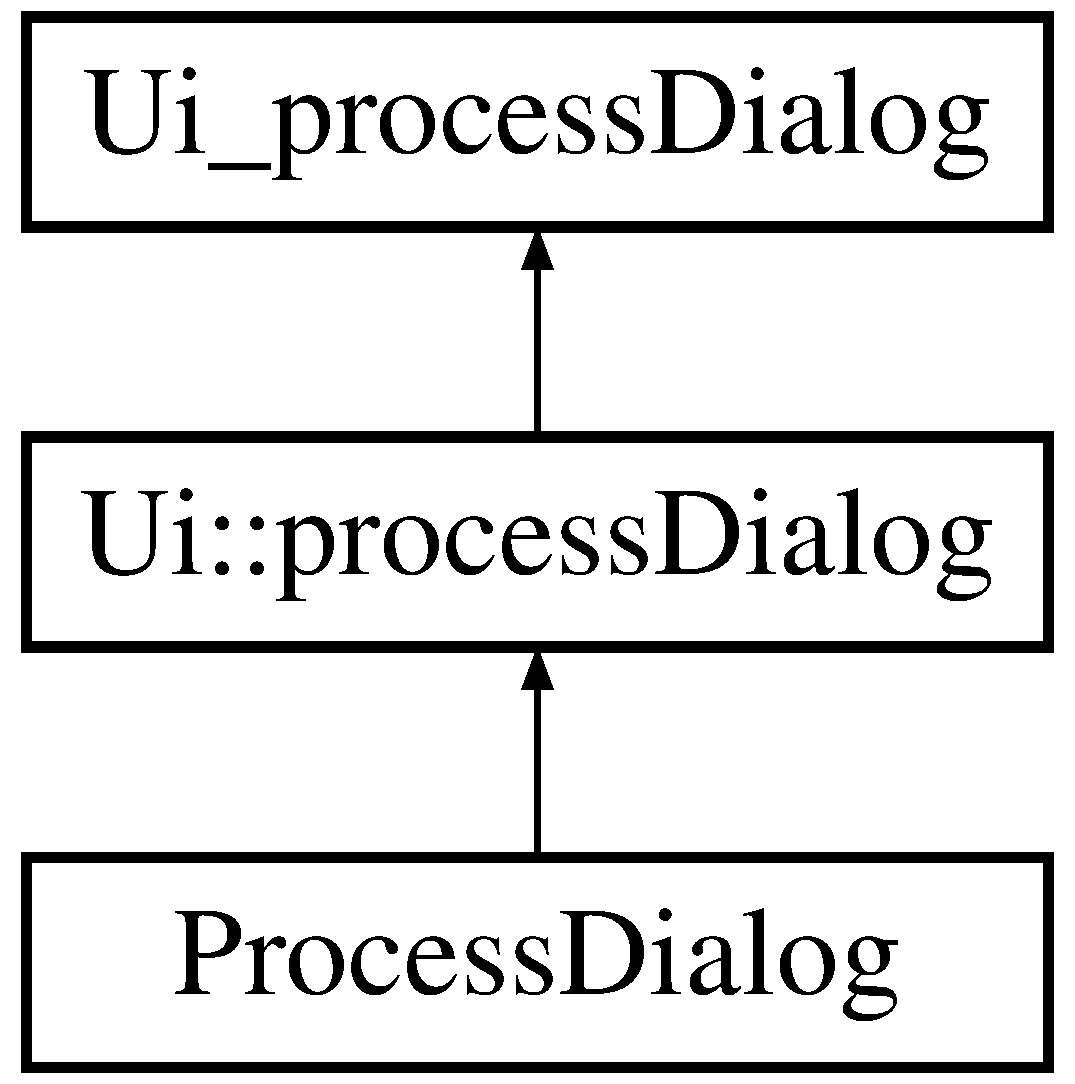
\includegraphics[height=3.000000cm]{class_ui__process_dialog}
\end{center}
\end{figure}
\subsection*{Public Member Functions}
\begin{DoxyCompactItemize}
\item 
\hypertarget{class_ui__process_dialog_add9ffd89cb5e2c1e3d3edd087f886eef}{
void {\bfseries setupUi} (QDialog $\ast$processDialog)}
\label{class_ui__process_dialog_add9ffd89cb5e2c1e3d3edd087f886eef}

\item 
\hypertarget{class_ui__process_dialog_a5cb554af240c0b999d38a211959ba826}{
void {\bfseries retranslateUi} (QDialog $\ast$processDialog)}
\label{class_ui__process_dialog_a5cb554af240c0b999d38a211959ba826}

\end{DoxyCompactItemize}
\subsection*{Public Attributes}
\begin{DoxyCompactItemize}
\item 
\hypertarget{class_ui__process_dialog_a66827385f230de1a247c233393d42a4c}{
QGridLayout $\ast$ {\bfseries gridLayout\_\-3}}
\label{class_ui__process_dialog_a66827385f230de1a247c233393d42a4c}

\item 
\hypertarget{class_ui__process_dialog_a6a72369b3dc2740c3830c7417521ae63}{
QLabel $\ast$ {\bfseries label}}
\label{class_ui__process_dialog_a6a72369b3dc2740c3830c7417521ae63}

\item 
\hypertarget{class_ui__process_dialog_ab933a0d256b6915f7b28701e724c08fa}{
QGroupBox $\ast$ {\bfseries groupBox}}
\label{class_ui__process_dialog_ab933a0d256b6915f7b28701e724c08fa}

\item 
\hypertarget{class_ui__process_dialog_afbd86e899c6b0976e799620569a18449}{
QGridLayout $\ast$ {\bfseries gridLayout\_\-2}}
\label{class_ui__process_dialog_afbd86e899c6b0976e799620569a18449}

\item 
\hypertarget{class_ui__process_dialog_a2196ade2f39330ae213922cb2408c7cc}{
QVBoxLayout $\ast$ {\bfseries verticalLayout\_\-9}}
\label{class_ui__process_dialog_a2196ade2f39330ae213922cb2408c7cc}

\item 
\hypertarget{class_ui__process_dialog_a0a56fe58abd4f07ab729ff42f2e9bde6}{
QVBoxLayout $\ast$ {\bfseries verticalLayout\_\-8}}
\label{class_ui__process_dialog_a0a56fe58abd4f07ab729ff42f2e9bde6}

\item 
\hypertarget{class_ui__process_dialog_adf64ec8b3747d17367e76eb14e8b7cd9}{
QLabel $\ast$ {\bfseries indicator\_\-label}}
\label{class_ui__process_dialog_adf64ec8b3747d17367e76eb14e8b7cd9}

\item 
\hypertarget{class_ui__process_dialog_a5ed0ac96dfe7e6d24a3f127089e064b1}{
QHBoxLayout $\ast$ {\bfseries horizontalLayout\_\-2}}
\label{class_ui__process_dialog_a5ed0ac96dfe7e6d24a3f127089e064b1}

\item 
\hypertarget{class_ui__process_dialog_afae559438bd7e27fa8ee67aa04c46409}{
QLabel $\ast$ {\bfseries channels\_\-label}}
\label{class_ui__process_dialog_afae559438bd7e27fa8ee67aa04c46409}

\item 
\hypertarget{class_ui__process_dialog_a45bca4f224e570163430cc183bf70808}{
QHBoxLayout $\ast$ {\bfseries horizontalLayout}}
\label{class_ui__process_dialog_a45bca4f224e570163430cc183bf70808}

\item 
\hypertarget{class_ui__process_dialog_ac70ab3f21858c52d94593b22cac779fa}{
QVBoxLayout $\ast$ {\bfseries verticalLayout\_\-2}}
\label{class_ui__process_dialog_ac70ab3f21858c52d94593b22cac779fa}

\item 
\hypertarget{class_ui__process_dialog_a9de0178d2b68ef65b50b4e73381e370b}{
QLabel $\ast$ {\bfseries channel1\_\-label}}
\label{class_ui__process_dialog_a9de0178d2b68ef65b50b4e73381e370b}

\item 
\hypertarget{class_ui__process_dialog_aecd5403cf06027fcd628a9470871d4f4}{
QCheckBox $\ast$ {\bfseries channel1\_\-box}}
\label{class_ui__process_dialog_aecd5403cf06027fcd628a9470871d4f4}

\item 
\hypertarget{class_ui__process_dialog_a4b900b7dccbbf9b44dd0ba84ccf318e6}{
QVBoxLayout $\ast$ {\bfseries verticalLayout\_\-3}}
\label{class_ui__process_dialog_a4b900b7dccbbf9b44dd0ba84ccf318e6}

\item 
\hypertarget{class_ui__process_dialog_a2d3c6488414604120f2871fbfc2e11ac}{
QLabel $\ast$ {\bfseries channel2\_\-label}}
\label{class_ui__process_dialog_a2d3c6488414604120f2871fbfc2e11ac}

\item 
\hypertarget{class_ui__process_dialog_a553437de75b83080addf2fa939f78af6}{
QCheckBox $\ast$ {\bfseries channel2\_\-box}}
\label{class_ui__process_dialog_a553437de75b83080addf2fa939f78af6}

\item 
\hypertarget{class_ui__process_dialog_a48b4e9e18550e4b0deab076f7807339f}{
QVBoxLayout $\ast$ {\bfseries verticalLayout\_\-4}}
\label{class_ui__process_dialog_a48b4e9e18550e4b0deab076f7807339f}

\item 
\hypertarget{class_ui__process_dialog_abc78c453a6ea0495c07c18e806b30d3e}{
QLabel $\ast$ {\bfseries channel3\_\-label}}
\label{class_ui__process_dialog_abc78c453a6ea0495c07c18e806b30d3e}

\item 
\hypertarget{class_ui__process_dialog_a925cf83c86cc7493e951ba9646266859}{
QCheckBox $\ast$ {\bfseries channel3\_\-box}}
\label{class_ui__process_dialog_a925cf83c86cc7493e951ba9646266859}

\item 
\hypertarget{class_ui__process_dialog_a5e7d2a1ffb5efb72b147dafb55dd2c89}{
QVBoxLayout $\ast$ {\bfseries verticalLayout\_\-5}}
\label{class_ui__process_dialog_a5e7d2a1ffb5efb72b147dafb55dd2c89}

\item 
\hypertarget{class_ui__process_dialog_a09322820269ab9f15a8dedfa555918ed}{
QLabel $\ast$ {\bfseries channel4\_\-label}}
\label{class_ui__process_dialog_a09322820269ab9f15a8dedfa555918ed}

\item 
\hypertarget{class_ui__process_dialog_a777865891f7303504448c6625b203415}{
QCheckBox $\ast$ {\bfseries channel4\_\-box}}
\label{class_ui__process_dialog_a777865891f7303504448c6625b203415}

\item 
\hypertarget{class_ui__process_dialog_af3eb901fdc36f88472927611ab30e509}{
QVBoxLayout $\ast$ {\bfseries verticalLayout\_\-6}}
\label{class_ui__process_dialog_af3eb901fdc36f88472927611ab30e509}

\item 
\hypertarget{class_ui__process_dialog_ae68d5e041d396564c1b1f21bf5ea12eb}{
QLabel $\ast$ {\bfseries channel5\_\-label}}
\label{class_ui__process_dialog_ae68d5e041d396564c1b1f21bf5ea12eb}

\item 
\hypertarget{class_ui__process_dialog_a9cb5f9edcebbfe405543f34dacb1dd72}{
QCheckBox $\ast$ {\bfseries channel5\_\-box}}
\label{class_ui__process_dialog_a9cb5f9edcebbfe405543f34dacb1dd72}

\item 
\hypertarget{class_ui__process_dialog_a74401838d86d91b07460f1d5d01c90c6}{
QVBoxLayout $\ast$ {\bfseries verticalLayout\_\-7}}
\label{class_ui__process_dialog_a74401838d86d91b07460f1d5d01c90c6}

\item 
\hypertarget{class_ui__process_dialog_ae25ebe8196fb3bd2094c5e85ab52a693}{
QLabel $\ast$ {\bfseries channel6\_\-label}}
\label{class_ui__process_dialog_ae25ebe8196fb3bd2094c5e85ab52a693}

\item 
\hypertarget{class_ui__process_dialog_a8a3035c2df405ba533ac36a22854e650}{
QCheckBox $\ast$ {\bfseries channel6\_\-box}}
\label{class_ui__process_dialog_a8a3035c2df405ba533ac36a22854e650}

\item 
\hypertarget{class_ui__process_dialog_a158c67863f0cb08474e8ede651cbbb5e}{
QSpacerItem $\ast$ {\bfseries verticalSpacer}}
\label{class_ui__process_dialog_a158c67863f0cb08474e8ede651cbbb5e}

\item 
\hypertarget{class_ui__process_dialog_ab72b7893a97b1cbdf9e31c2c0d9bd3f0}{
QHBoxLayout $\ast$ {\bfseries horizontalLayout\_\-4}}
\label{class_ui__process_dialog_ab72b7893a97b1cbdf9e31c2c0d9bd3f0}

\item 
\hypertarget{class_ui__process_dialog_a293ba980bc67923d60a21bc41cfe88fe}{
QVBoxLayout $\ast$ {\bfseries verticalLayout}}
\label{class_ui__process_dialog_a293ba980bc67923d60a21bc41cfe88fe}

\item 
\hypertarget{class_ui__process_dialog_af8c91a7266d93e846256e124a4183985}{
QLabel $\ast$ {\bfseries zone\_\-length\_\-label}}
\label{class_ui__process_dialog_af8c91a7266d93e846256e124a4183985}

\item 
\hypertarget{class_ui__process_dialog_ab67d9fa3241aa8d05b479ca4ce87cf45}{
QSpinBox $\ast$ {\bfseries zone\_\-length\_\-spin}}
\label{class_ui__process_dialog_ab67d9fa3241aa8d05b479ca4ce87cf45}

\item 
\hypertarget{class_ui__process_dialog_a734a2be679589ebc7e31c9da8a1dd891}{
QHBoxLayout $\ast$ {\bfseries horizontalLayout\_\-3}}
\label{class_ui__process_dialog_a734a2be679589ebc7e31c9da8a1dd891}

\item 
\hypertarget{class_ui__process_dialog_a083e9e4b4acfe497522501f311b8249f}{
QLabel $\ast$ {\bfseries scale\_\-label}}
\label{class_ui__process_dialog_a083e9e4b4acfe497522501f311b8249f}

\item 
\hypertarget{class_ui__process_dialog_a0443beb314621cbf9123ce933b816ce1}{
QLabel $\ast$ {\bfseries scale\_\-value\_\-label}}
\label{class_ui__process_dialog_a0443beb314621cbf9123ce933b816ce1}

\item 
\hypertarget{class_ui__process_dialog_a8af5b9b4156e415f7e81d68d82f8398d}{
QSpacerItem $\ast$ {\bfseries horizontalSpacer}}
\label{class_ui__process_dialog_a8af5b9b4156e415f7e81d68d82f8398d}

\item 
\hypertarget{class_ui__process_dialog_a94114aa89f42109d7c7c9dad6f9d0ea8}{
QTableWidget $\ast$ {\bfseries display\_\-table}}
\label{class_ui__process_dialog_a94114aa89f42109d7c7c9dad6f9d0ea8}

\item 
\hypertarget{class_ui__process_dialog_a69629897a20490527c5f0792402ce156}{
QTabWidget $\ast$ {\bfseries tabWidget}}
\label{class_ui__process_dialog_a69629897a20490527c5f0792402ce156}

\item 
\hypertarget{class_ui__process_dialog_a88018eaf7308f1e438e5fb3b461b66ee}{
QWidget $\ast$ {\bfseries tab}}
\label{class_ui__process_dialog_a88018eaf7308f1e438e5fb3b461b66ee}

\item 
\hypertarget{class_ui__process_dialog_ae4354dca860d721ac48a68e530931386}{
QGridLayout $\ast$ {\bfseries gridLayout}}
\label{class_ui__process_dialog_ae4354dca860d721ac48a68e530931386}

\item 
\hypertarget{class_ui__process_dialog_abf2e5008b182cbee2f4735a710a42f92}{
QwtPlot $\ast$ {\bfseries plot}}
\label{class_ui__process_dialog_abf2e5008b182cbee2f4735a710a42f92}

\item 
\hypertarget{class_ui__process_dialog_a81c8da6ac87cb40cf59830091014beac}{
QWidget $\ast$ {\bfseries tab\_\-2}}
\label{class_ui__process_dialog_a81c8da6ac87cb40cf59830091014beac}

\item 
\hypertarget{class_ui__process_dialog_a2d8294d876cfc86f5a76784ce3c2897c}{
QPushButton $\ast$ {\bfseries stopButton}}
\label{class_ui__process_dialog_a2d8294d876cfc86f5a76784ce3c2897c}

\end{DoxyCompactItemize}


The documentation for this class was generated from the following file:\begin{DoxyCompactItemize}
\item 
ui\_\-processdialog.h\end{DoxyCompactItemize}

\printindex
\end{document}
